% Generated by build.py (latex.py) from sections/*.md - do not edit; edit the sections and rebuild.
% Needs a Unicode engine: tectonic paper.tex, or xelatex/lualatex (twice, for the cross-references).
\documentclass[10pt,letterpaper]{article}
\usepackage[letterpaper,hmargin=1.05in,vmargin=1in]{geometry}
\usepackage{amsmath,amssymb}
\usepackage{fontspec}
\defaultfontfeatures[\rmfamily,\sffamily]{}% no TeX ligatures: "--" is two hyphens, quotes are already curled
\setmainfont{LibertinusSerif}[Extension=.otf,UprightFont=*-Regular,BoldFont=*-Bold,
  ItalicFont=*-Italic,BoldItalicFont=*-BoldItalic]
\setmonofont{DejaVuSansMono}[Extension=.ttf,UprightFont=*,BoldFont=*-Bold,
  ItalicFont=*-Oblique,BoldItalicFont=*-BoldOblique,Scale=0.78]
\usepackage{microtype}
\usepackage{graphicx,xcolor}
\usepackage{booktabs,array,tabularx,longtable}
\usepackage{enumitem}
\usepackage[colorlinks=true,linkcolor=black,citecolor=black,urlcolor=blue!45!black,
  pdftitle={Frozen-Grid Re-Rounding and the Limits of Low-Rank Correction for llama.cpp Quantization: A Paired Audit},pdfauthor={Maximilian Khan}]{hyperref}
\setlength{\parindent}{0pt}
\setlength{\parskip}{0.62em plus 0.1em minus 0.05em}
\setlist[itemize]{leftmargin=1.5em,itemsep=0.25em,topsep=0.1em,parsep=0pt}
\setlength{\emergencystretch}{2em}
\renewcommand{\arraystretch}{1.12}
\makeatletter
\renewcommand\section{\@startsection{section}{1}{\z@}{-1.6em plus -.3em}{0.5em}{\normalfont\fontsize{13}{15.5}\selectfont\bfseries\raggedright}}
\renewcommand\subsection{\@startsection{subsection}{2}{\z@}{-1.1em plus -.2em}{0.3em}{\normalfont\fontsize{11}{13.5}\selectfont\bfseries\raggedright}}
\makeatother
\newcommand{\src}[1]{{\fontsize{7.5}{9}\selectfont\color{black!57}\ [#1]}}
\title{\fontsize{15}{18.5}\selectfont\bfseries Frozen-Grid Re-Rounding and the Limits of Low-Rank Correction for llama.cpp Quantization: A Paired Audit}
\author{\normalsize\fontsize{11}{14}\selectfont Maximilian Khan\\[0.3em]
  \footnotesize\color{black!69}OpenBeast project · \href{https://github.com/MaximilianKhan/openbeast}{github.com/MaximilianKhan/openbeast}}
\date{\footnotesize\color{black!69}October 2026}
\begin{document}
\maketitle
\begin{abstract}
\noindent We measure, on llama.cpp files of four Qwen-family models and one GPU, what post-training repair of low-bit quantization buys. (1) Frozen-grid re-rounding re-chooses only the codes on llama-quantize’s grids. At identical bytes it lowers a Q2\_K file’s KL divergence (KLD) by 34\% at 0.8B and 13\% at 27B (legacy-provenance pair; perplexity unchanged; no held-out test). Calibrated on one corpus it harms a distant one; mixed calibration repairs this. The smaller stock IQ3\_XXS file still beats re-rounded Q2\_K at 0.8B. (2) At 27B, whitened low-rank correction is ahead of the adjacent stock type by 0.0048 KLD (5\%, t = −2.85) and behind a same-byte mixed-type control by 0.0063 (t = +2.62); both margins are small, on-distribution and unreplicated. (3) Against released GSQ-RCO checkpoints, the untrained baseline at matched bytes already has lower 512-token KLD on wikitext; our correction (+0.9 GB) lowers it further, and a stock file at near-equal bytes beats it. In one pair, one run per arm, KLD and a coding suite ordered the files oppositely. (4) Fused adapter kernels raise 0.6B decode by 79\% (one pair, one GPU); an allocator fix adds 19.6\% in the better of two sessions (11\% in the other) and nothing at 27B\src{E35, E32, E25}.
\end{abstract}

\section*{\phantomsection\label{sec:1}1\hspace{0.8em}Introduction}
\addcontentsline{toc}{section}{1. Introduction}

\subsection*{\phantomsection\label{sec:1.1}1.1\hspace{0.8em}The setting}
\addcontentsline{toc}{subsection}{1.1 The setting}

A consumer GPU such as the RTX 5090 pairs a fast processor with 32 GB of memory, and the models people want to run on it are several times larger than that at training precision. Single-stream decoding is limited by memory bandwidth, because every token reads the full weight set. We measured the consequence on one 27B model, Qwen3.6-27B (the checkpoint is heretic-v2, an uncensored community finetune of Qwen3.6-27B that keeps the base model’s multi-token-prediction layers): the Q6\_K file occupies 23.6 GB of VRAM and decodes at 61 tok/s, and the Q2\_K file occupies 13.0 GB and decodes at 99.7 tok/s\src{rollup}. On this card, for these two files, the smaller one was also the faster one. We take that as the motivation for the study and not as a general result.

The question is how much quality post-training processing can recover per byte, or at zero added bytes, on top of a mature quantization stack. We ask it on llama.cpp, whose family of imatrix-weighted block quantizers (the K-quant and I-quant types, nominally about 1.5 to 6.5 bits per weight; terms are defined in \hyperref[sec:2]{§2}) is the strongest deployed baseline in this regime and a harder rival than round-to-nearest. All models are Qwen-family and all measurements come from one GPU.

\subsection*{\phantomsection\label{sec:1.2}1.2\hspace{0.8em}What this paper does not claim}
\addcontentsline{toc}{subsection}{1.2 What this paper does not claim}

It does not claim that low-rank factorization compresses these models. A singular-value census of every tensor in our smallest model finds that capturing 95\% of unweighted Frobenius energy needs 50-80\% of full rank on every projection type\src{E1}. The quantization residual R = W − dequant(Q), the object that the error-correction lineage corrects (ZeroQuant-V2/LoRC, \cite{arxiv2303.08302}; LQER, \cite{arxiv2402.02446}; QERA, \cite{arxiv2410.06040}; EoRA, \cite{arxiv2410.21271}; CALDERA, \cite{arxiv2405.18886}), is less structured still: 90\% of its energy needs about 62\% of full rank\src{E3}. Both observations agree with the published account (LQER; RILQ, \cite{arxiv2412.01129}).

It does not claim a method that beats llama.cpp’s stock quantization types. At 100 chunks (the pre-registered final sample, after ties at 20 and 40) the corrected configuration is ahead of Q3\_K\_S by 0.0048 KLD (5\%, t = −2.85, 71/100 chunks) and behind a same-byte mixed-type control by 0.0063 (t = +2.62, 62/100; no difference in NLL). Both margins are small, on-distribution, and unreplicated. The registration fixed n = 100 as final and stated a rule for parity (|t| < 2); it stated no rule for a win and no correction for the three looks. The I-quant type IQ3\_XS scores better than both at fewer bytes with no adapter (\hyperref[sec:4.3]{§4.3})\src{E27, E35}.

\subsection*{\phantomsection\label{sec:1.3}1.3\hspace{0.8em}Contributions}
\addcontentsline{toc}{subsection}{1.3 Contributions}

\textbf{(1) Frozen-grid re-rounding, conditioned on calibration breadth.} llama-quantize chooses a grid per block and then rounds each element independently. We keep the grid bytes as shipped and re-choose only the codes under a captured activation-covariance metric, using the GPTQ sweep (\cite{arxiv2210.17323}). The output is a standard GGUF of identical size. Against the same file before re-rounding, Qwen3.5-0.8B at Q2\_K improves by 15\% in perplexity and 34\% in KL divergence (paired NLL t = −44.9, n = 580; paired KLD t = −30.3, n = 40)\src{E24}. At 27B the same sweep lowers KL divergence by 13.3\% (t = −7.0, n = 100; a legacy-provenance pair; perplexity unchanged; no held-out test at 27B).

Three limits belong with that result. Re-rounding improves a given file and does not make Q2\_K the best choice at its size: at 0.8B the stock IQ3\_XXS file is smaller and has lower KL divergence (\hyperref[sec:3.1]{§3.1}). The gain depends on calibration: the wikitext-calibrated file is worse than the untouched one on a held-out code corpus, and a mixed calibration improves both corpora. And the tool needs the higher-precision source weights and a covariance capture made with a patched binary; it does not operate on a GGUF alone. Related methods are GSQ (\cite{arxiv2604.18556}), ReQuant (\cite{arxiv2608.07019}) and SchurQuant (\cite{arxiv2608.15567}); the relation is stated in \hyperref[sec:8]{§8}.

\textbf{(2) A paired audit of low-rank correction on llama.cpp’s own formats, with the reasons it falls short.} We measure whitened low-rank correction at three dense sizes and on one mixture-of-experts model, against the stock types and, at 27B and on the mixture-of-experts model, against a mixed-type control built at the same bytes. The correction improves its own base at every size and loses to the control where one was built. Three placements of the low-rank bytes cannot be told apart at 27B, within a bound we state (\hyperref[sec:4.4]{§4.4}). Fixed-rank capture is sublinear in rank and, across a single width step, falls more slowly than r/d predicts (\hyperref[sec:4.2]{§4.2}). Several of the audit’s negative results are its best-resolved findings (\hyperref[sec:4.7]{§4.7}, Appendix A)\src{review}.

\textbf{(3) A head-to-head with released trained checkpoints.} Against the released GSQ-RCO checkpoints of Qwen3.8-27B, the untrained vendor baseline at matched bytes already has lower 512-token KLD on wikitext (not resolved on FineWeb-Edu); adding our correction (+0.9 GB, not byte-matched) lowers it further on both corpora. A stock file at near-equal total bytes beats the corrected arm. In one cross-family pair (one run per arm), 512-token KLD and a coding suite ordered the artifacts oppositely; we treat KLD as unvalidated across refinement families (\hyperref[sec:5]{§5}).

\textbf{(4) Serving kernels.} llama.cpp’s stock adapter path costs 20-40\% of decode speed. A fused-kernel series removes most of that at 0.6B (+79\%, one same-session pair) and gives +2.7\% at 27B (N = 10, interleaved). A separate allocator fix raised base decode at 0.6B by 19.6\% in the better of two sessions and 11\% in the other, with no measurable change at 27B (\hyperref[sec:6]{§6})\src{E14, E25}.

The measurement protocol these results follow (single-step provenance, paired per-chunk statistics, a same-byte control, pre-registration) is part of the method and is stated in \hyperref[sec:2.5]{§2.5}.

\subsection*{\phantomsection\label{sec:1.4}1.4\hspace{0.8em}Relation to prior work}
\addcontentsline{toc}{subsection}{1.4 Relation to prior work}

The pipeline is assembled from published mathematics: QERA’s whitened closed forms, LoftQ’s alternation, and GPTQ’s sweep on a frozen grid. What we add is where it is measured: on llama.cpp’s deployed formats, against its stock types and a same-byte mixed-type control, with paired statistics. \hyperref[sec:8]{§8} gives the comparison in full.

The paper follows the pipeline: method (\hyperref[sec:2]{§2}), re-rounding (\hyperref[sec:3]{§3}), the correction audit (\hyperref[sec:4]{§4}), the GSQ-RCO head-to-head (\hyperref[sec:5]{§5}), serving (\hyperref[sec:6]{§6}), limitations (\hyperref[sec:7]{§7}), related work (\hyperref[sec:8]{§8}). Appendix A holds additional negative results.

\section*{\phantomsection\label{sec:2}2\hspace{0.8em}Method}
\addcontentsline{toc}{section}{2. Method}

The pipeline has four stages: capture second-moment statistics on calibration text (\hyperref[sec:2.1]{§2.1}); fit whitened corrections in closed form (\hyperref[sec:2.2]{§2.2}) or re-round the base’s codes on their frozen grids (\hyperref[sec:2.3]{§2.3}); optionally alternate quantizer and corrector (\hyperref[sec:2.4]{§2.4}); serve through llama.cpp’s adapter path or our fused kernels (\hyperref[sec:6]{§6}). Quality claims follow the measurement protocol of \hyperref[sec:2.5]{§2.5}.

\textbf{Terms.} The \emph{imatrix} is llama.cpp’s importance statistic: for each weight column, the mean squared input activation on calibration text, which llama-quantize uses to weight its rounding error. \emph{K-quants} (Q2\_K, Q3\_K\_S, Q3\_K\_M, Q4\_K\_M, Q6\_K) are llama.cpp’s block-wise scalar quantizers; the digit is the nominal bit width of the main tensor type and the suffix (S, M) says how many tensors are promoted to a wider type. \emph{I-quants} (IQ1\_S, IQ2\_XS, IQ3\_XXS, IQ3\_XS) are its codebook-based types at similar or smaller sizes. We call the set of stock types ordered by file size \emph{the ladder} and one stock type \emph{a rung}. \emph{UD} marks Unsloth Dynamic files, vendor quantizations that choose a type per tensor. \emph{MTP} is the multi-token-prediction head some of these checkpoints carry; we pin its tensors to a fixed type. \emph{GDN} is Gated DeltaNet, the linear-attention layer of the hybrid architecture (llama.cpp name \texttt{qwen35}) used by Qwen3.5-0.8B and Qwen3.8-27B. The sizes of the types used at 27B, each one quantization step from BF16\src{E27}:

\begin{center}\fontsize{8.5}{10.5}\selectfont\setlength{\tabcolsep}{4pt}
\begin{tabular}{@{}lll@{}}
\toprule
\textbf{type} & \textbf{file GB (Qwen3.6-27B)} & \textbf{bits per weight (file bytes × 8 / parameters)} \\
\midrule
Q2\_K & 11.00 & 3.22 \\
IQ3\_XXS & 11.48 & 3.36 \\
IQ3\_XS & 12.26 & 3.59 \\
Q3\_K\_S & 12.37 & 3.62 \\
Q3\_K\_M & 13.59 & 3.98 \\
Q4\_K\_M & 16.84 & 4.93 \\
\bottomrule
\end{tabular}
\end{center}

A nominal “Q2\_K” file is above 3 bits per weight because llama-quantize promotes some tensors to wider types. Bits per weight in this paper are file bytes over parameter count unless marked nominal.

\textbf{Configurations.} We use four names throughout. \emph{Re-rounding} is the code re-selection of \hyperref[sec:2.3]{§2.3}. \emph{Full-covariance correction} is the low-rank adapter of \hyperref[sec:2.2]{§2.2} whitened by the full input Gram, as opposed to the imatrix diagonal. \emph{The mixed base} is the 27B base with FFN tensors at Q3\_K and the remaining tensors at Q2\_K. \emph{The corrected configuration} is a base plus its correction; at 27B it means the mixed base plus a rank-128 full-covariance correction with Q8\_0 factors on the non-FFN tensors. \emph{The control} is a file with no adapter, built from stock tensor types at the corrected configuration’s byte count.

\subsection*{\phantomsection\label{sec:2.1}2.1\hspace{0.8em}Statistics capture}
\addcontentsline{toc}{subsection}{2.1 Statistics capture}

\textbf{Input-side Grams.} llama-imatrix accumulates diag(E[x²]) per weight column, which is the diagonal scaling used by LQER (\cite{arxiv2402.02446}) and QERA-approx (\cite{arxiv2410.06040}). We extended it (a local, environment-gated C++ patch of about 140 lines) to accumulate the full Gram G = Σ x x\textsuperscript{T} per distinct layer input: one for the attention q/k/v input, one for the FFN gate/up input, one each for attn\_output and ffn\_down. Accumulation is fp32. The diagonal of the captured Gram matches the stock imatrix to a median relative error of 2e-8, and the matrices are symmetric and positive semidefinite\src{E10}. Inputs wider than 8,192 dimensions are captured block-diagonally in 8 blocks, an approximation forced by memory whose consequence is stated in \hyperref[sec:2.2]{§2.2}.

\textbf{Mixture-of-experts extension.} The expert-routed branch needs its own accumulator, because rows from different experts are mixed and must be unpacked per (token, slot) pair. We capture one pooled Gram per expert stack, the union of routed inputs, and not a Gram per expert: at 16 calibration chunks there are about 256 samples per expert for a 2,048-dimensional Gram, which is rank-deficient, while the pooled Gram is full-rank. The validation gates pass on Qwen3.6-35B-A3B\src{E23}.

\textbf{Output-gradient Grams.} For two-sided metrics we built llama-gradmatrix, which runs llama.cpp’s training loop forward and backward with learning disabled and captures T = Σ g g\textsuperscript{T} per tensor, where g is the loss gradient at the output row. Two repairs were needed. llama.cpp’s trainer does not backpropagate through the KV cache (upstream issue \#21037 reports the same gap), which we bypass by feeding k/v directly to attention when the window is one micro-batch. Several operations of the GDN layers have no backward pass, which we handle with an explicit gradient cut that stops flow through those layers’ token mixing and keeps the residual path. At 0.8B the cut biases the 18 linear-attention layers, which matters in \hyperref[sec:3.2]{§3.2}\src{E20}.

\subsection*{\phantomsection\label{sec:2.2}2.2\hspace{0.8em}Whitened low-rank correction}
\addcontentsline{toc}{subsection}{2.2 Whitened low-rank correction}

Given the residual R = W\_ref − dequant(Q) and a whitener L (the damped Cholesky factor of G/count; damping 0.01 × mean diagonal, the convention of \cite{arxiv2210.17323} and \cite{arxiv2501.18475}; the route is numerically viable at this size by \cite{arxiv2403.07378}), the rank-r corrector minimizes the activation-weighted error ‖(R − Δ) L‖\_F². The two-sided weighted problem is NP-hard (\cite{arxiv1012.0197}); the one-sided problem has a closed form: whiten, truncate, unwhiten. It is the L\_g = I case of the two-sided objective of OBD-LLM (\cite{arxiv2604.00821}). We stay one-sided for three reasons: a tool that starts from a shipped file has no gradients; a diagonal output weighting provably cannot change a frozen-grid rounding decision (\hyperref[sec:2.3]{§2.3}); and the published two-sided gain is on weight decomposition at 8B, not on residual correction of K-quant grids\src{theory-L6}.

We use the projection form: B = U\_r, the top-r left singular vectors of R L, and A = B\textsuperscript{T} R. For any invertible right whitener the unwhitening factor cancels, so this is the exact optimum; our code check agrees with the explicit argmin to 7e-15\src{review}. Factors are computed by randomized SVD (\cite{arxiv0909.4061}; oversampling 32, 4 power iterations).

\textbf{The blocked-whitening caveat.} For inputs above 8,192 dimensions the captured Gram is block-diagonal. At 27B this applies to ffn\_down, whose input has 17,408 dimensions (8 blocks of 2,176). The projection form is then optimal for the block-diagonal surrogate and not for the true E[xx\textsuperscript{T}]; a synthetic test with cross-block correlation measured a 25\% excess of true-metric loss for the blocked optimum\src{review}. Every “full-covariance” 27B row therefore means full covariance for inputs up to 8,192 dimensions and 8-block-diagonal for ffn\_down. End-to-end measurements score the artifact and are unaffected; the mechanism claim that the metric was the bottleneck is untested against a truly full metric at that width.

\textbf{Two-sided variant.} With both S and T captured, B = L\_T\textsuperscript{-\textsuperscript{T}} U\_r and A is solved against L\_S, with a factor-balancing step that leaves the product unchanged and prevents half-precision overflow\src{review}.

\textbf{Factor density.} Factors are stored as Q8\_0 (llama.cpp’s 8-bit block format), which halves their bytes at measured quality parity (rank 64 with Q8\_0 factors: perplexity 31.26 against 31.29 with F16 factors at 0.6B), the observation of \cite{arxiv2406.08903} and \cite{arxiv2303.08302} confirmed in this pipeline\src{journal}.

\textbf{Serving and what is not stock.} The corrected model is a quantized base GGUF plus a LoRA-form adapter GGUF, and y = Q·x + s·B·(A·x) is llama.cpp’s stock adapter path. The artifact therefore serves on an unmodified llama-server, at the decode cost \hyperref[sec:6]{§6} measures. Capture is not stock: every full-covariance number depends on our Gram patch to llama-imatrix, and gradient Grams on llama-gradmatrix.

\subsection*{\phantomsection\label{sec:2.3}2.3\hspace{0.8em}Re-rounding on frozen grids}
\addcontentsline{toc}{subsection}{2.3 Re-rounding on frozen grids}

A K-quant tensor stores, per 16-element sub-block, a scale and offset (the grid) and a low-bit code per element. llama-quantize chooses both and rounds each element independently. We keep the grid bytes exactly as written and re-choose only the codes to minimize the whitened objective of \hyperref[sec:2.2]{§2.2} with Δ = 0, which is a closest-vector problem on the frozen grid. The solver is the GPTQ error-feedback sweep: process columns in order, round the current column on its grid, and propagate the scaled error to the unprocessed columns through the upper-triangular Cholesky factor of the inverse Gram. With frozen grids the objective does not increase from sweep to sweep (\cite{arxiv2606.01412}).

The objective needs W\_ref, the higher-precision weights, and the Gram, which is captured on the patched binary. The method therefore starts from a model’s source weights plus a calibration pass, and writes a file that is byte-compatible with the stock one: same size, same type tags, loadable by any llama.cpp build.

Two related methods work the same quadratic. ReQuant (\cite{arxiv2608.07019}) performs cyclic coordinate descent on it outside the GGUF format, and SchurQuant (\cite{arxiv2608.15567}) also refits the scales\src{theory-L6}.

Implementation points that affect the numbers: the Q2\_K codec was mirrored from gguf-py and round-trips real tensors byte-identically; the triangular convention matters (a lower factor disables the feedback and reproduces llama-quantize’s codes exactly); and Cholesky failures escalate damping\src{E13}. Only the Q2\_K codec is implemented. A two-sided (Kronecker) generalization of the sweep is derived and tested in the experiment record, together with a small negative result: a diagonal output-side weighting cannot change any code, because each row’s argmin is scale-invariant\src{E24}.

\subsection*{\phantomsection\label{sec:2.4}2.4\hspace{0.8em}Alternation}
\addcontentsline{toc}{subsection}{2.4 Alternation}

Correction quality depends on the base, and the base’s grid choices depend on what the corrector will absorb. We alternate Q\_\{t+1\} = quant(W − C\_t) and C\_\{t+1\} = corr(W − Q\_\{t+1\}), which is LoftQ’s template (\cite{arxiv2310.08659}) with llama-quantize as a black-box quantizer and the whitened closed form as the corrector, and we keep the best iterate and stop when a round is worse. Because the quantizer’s output set is finite and the corrector step is an exact minimum, the best-iterate value is non-increasing and becomes constant after finitely many rounds. In practice two or three rounds are used and later changes are below noise. The argument, its measured amendment (iterates settle onto a small limit cycle and not a fixed point), and the pointers to related metric-modification schemes are in Appendix A.5\src{theory-alt}.

\subsection*{\phantomsection\label{sec:2.5}2.5\hspace{0.8em}Measurement protocol}
\addcontentsline{toc}{subsection}{2.5 Measurement protocol}

Results in \hyperref[sec:3]{§3}-\hyperref[sec:6]{§6} follow these rules or are labeled legacy\src{protocol}.

\begin{itemize}
\item\relax \textbf{Reference and provenance.} The reference is BF16 where it exists. For the mixture-of-experts model of \hyperref[sec:4.6]{§4.6} we had no BF16 and used the vendor UD-Q4\_K\_M file, stated at the table. Every base and adapter derives from the reference in one quantization step; rows of other provenance are labeled legacy and are not tabled beside single-step rows without a provenance label.
\item\relax \textbf{Metrics.} Mean KL divergence (KLD) and top-1 agreement against reference logits at a 512-token context, on at least 40 chunks (100 for the 27B comparison of \hyperref[sec:4.3]{§4.3}; 20 for the mixture-of-experts table and some legacy rows), with standard errors. KLD is used because it tracks answer flips (\cite{arxiv2407.09141}) and is the measure llama.cpp’s maintainers use (discussion \#4110). Full-corpus perplexity is secondary (\cite{arxiv2606.19558}).
\item\relax \textbf{Paired statistics.} Compared files share evaluation tokens and reference logits. A comparison is decided by the per-chunk difference: its mean, standard error and t. We write t for a paired statistic with n − 1 degrees of freedom, where n is the chunk count given with it, and we reserve “standard errors” for unpaired distances, labeled as such.
\item\relax \textbf{What the t statistics are conditional on.} All intervals are conditional on one calibration sample and one evaluation corpus; they quantify evaluation-chunk variance only. An accidental control put calibration-sampling variance at 0.55 perplexity points (about 2\%) at 0.8B, which is larger than several small-scale margins (\hyperref[sec:3.1]{§3.1}).
\item\relax \textbf{Multiplicity.} No family-wise correction was applied across the paper’s contrasts, so margins near |t| = 2-3 are suggestive and not confirmatory.
\item\relax \textbf{Dependence between chunks.} Adjacent 512-token chunks of one corpus are not independent. For the load-bearing pairs we report, in addition to t, an exact sign test, a Wilcoxon signed-rank test, and a bootstrap over contiguous blocks of 10 chunks\src{E35}.
\item\relax \textbf{Byte-fair comparison.} Total bytes are base plus adapter. A comparison against the ladder includes K-quants, I-quants, and where built a mixed-type control at the matched byte count.
\item\relax \textbf{Speed.} Same-session A/B pairs only. Between-session drift on identical configurations reached 9\%.
\item\relax \textbf{Pre-registration.} From the second internal review onward, each experiment’s configuration, pairs and decision rules were written to the project journal with a timestamp before the run. The journal is the project’s own record and has not been audited externally.
\item\relax \textbf{Claims.} We call a relation a law only with at least three scale points and a stated functional form; otherwise it is an observation.
\end{itemize}

\section*{\phantomsection\label{sec:3}3\hspace{0.8em}Results I: re-rounding at zero added bytes}
\addcontentsline{toc}{section}{3. Results I: re-rounding at zero added bytes}

\subsection*{\phantomsection\label{sec:3.1}3.1\hspace{0.8em}What re-rounding changes, and what it does not}
\addcontentsline{toc}{subsection}{3.1 What re-rounding changes, and what it does not}

Re-rounding changes no file size, VRAM use or serving speed: it re-chooses which available code each weight gets, using one calibration pass and the model’s higher-precision source weights. It improves a given K-quant file at zero bytes; it does not make Q2\_K the best choice at its byte point. We report three sizes, and at each we add the stock rung nearest in size.

\textbf{Qwen3-0.6B (Q2\_K with imatrix; legacy scoring against a Q8\_0 reference).}\src{E13}

\begin{center}\fontsize{8.5}{10.5}\selectfont\setlength{\tabcolsep}{4pt}
\begin{tabular}{@{}llll@{}}
\toprule
\textbf{file (296 MB)} & \textbf{PPL} & \textbf{KLD} & \textbf{top-1} \\
\midrule
Q2\_K, as written by llama-quantize & 43.33 & 0.766 & 58.2\% \\
Q2\_K, re-rounded & 35.54 & 0.556 & 64.0\% \\
\bottomrule
\end{tabular}
\end{center}

Perplexity falls by 18\%. The two rows are 15.6 unpaired standard errors apart on perplexity and about 19 on KLD\src{E35}. No per-chunk logs exist for this pair, and no smaller stock rung was scored against it.

\textbf{Qwen3.5-0.8B (Q2\_K; BF16 reference; paired).} A second, hybrid-attention architecture\src{E24, E22}:

\begin{center}\fontsize{8.5}{10.5}\selectfont\setlength{\tabcolsep}{4pt}
\begin{tabular}{@{}lllll@{}}
\toprule
\textbf{file} & \textbf{MB} & \textbf{PPL} & \textbf{KLD} & \textbf{top-1} \\
\midrule
Q2\_K, as written & 436 & 33.09 & 0.4902 & 66.4\% \\
Q2\_K, re-rounded & 436 & 28.09 & 0.3234 & 72.7\% \\
IQ3\_XXS, stock & 412 & 23.95 & 0.2573 & 74.3\% \\
Q3\_K\_M, stock & 480 & 23.28 & 0.1668 & 79.2\% \\
\bottomrule
\end{tabular}
\end{center}

Re-rounded against the same file as written: ΔNLL −0.1637 ± 0.0036 nats/token (t = −44.9, n = 580, better on 557 chunks), ΔKLD −0.1668 ± 0.0055 (t = −30.3, n = 40, better on 40), Δtop-1 +6.26 ± 0.45 points (t = +14.1, n = 40). That is 15\% lower perplexity and 34\% lower KLD at identical bytes, and about half of the KLD distance to Q3\_K\_M (51.6\%).

Re-rounded Q2\_K against the stock IQ3\_XXS file, which is 24 MB smaller: the stock file is better, by 0.0657 ± 0.0061 KLD (t = +10.8, n = 40, IQ3\_XXS better on 39 chunks; Wilcoxon p < 1e-11), by 0.136 nats/token in NLL (t = +11.5) and by 1.6 points of top-1 (t = −3.1). The two logs come from different sessions and were scored against the same 40-chunk BF16 reference, which we verified by recovering the reference’s per-chunk NLL from each log\src{E35}. At 0.8B, then, a user choosing a file near 430 MB should take the stock IQ3\_XXS over a re-rounded Q2\_K. Whether re-rounding would improve IQ3\_XXS in turn is not known, because the re-rounder implements only the Q2\_K codec.

\textbf{Qwen3.6-27B (Q2\_K with imatrix; paired, n = 100; legacy-provenance pair).} On 100 chunks against BF16 reference logits\src{E27}:

\begin{center}\fontsize{8.5}{10.5}\selectfont\setlength{\tabcolsep}{4pt}
\begin{tabular}{@{}llllll@{}}
\toprule
\textbf{file} & \textbf{GB} & \textbf{n} & \textbf{PPL} & \textbf{KLD} & \textbf{top-1} \\
\midrule
Q2\_K, as written (legacy provenance) & 10.86 & 100 & 7.735 ± 0.126 & 0.1603 ± 0.0032 & 83.48\% \\
Q2\_K, re-rounded (legacy provenance) & 10.86 & 100 & 7.696 ± 0.124 & 0.1390 ± 0.0029 & 84.55\% \\
IQ3\_XXS, stock (single step from BF16) & 11.48 & 20 & 7.562 ± 0.270 & 0.0983 ± 0.0041 & 87.29\% \\
\bottomrule
\end{tabular}
\end{center}

Re-rounded against as written: ΔKLD −0.0213 ± 0.0030 (t = −7.02, better on 77/100 chunks; block-bootstrap 95\% interval [−0.0285, −0.0138]; Wilcoxon p < 1e-10), Δtop-1 +1.07 points (t = +4.72), ΔNLL −0.005 ± 0.005 (t = −0.98). KL divergence falls by 13.3\% and perplexity does not move.

Three labels travel with this pair wherever it is quoted. It is legacy provenance: both files are requantizations of a Q6\_K file and not single steps from BF16, so the pair is not tabled beside the single-step rows of \hyperref[sec:4.3]{§4.3}; the difference between the two is clean because both share that provenance. Perplexity is unchanged. And there is no held-out test of the re-rounder at 27B. In addition, the sweep covers part of the model: inside a nominal Q2\_K file at 27B, llama-quantize writes ffn\_down and attn\_output as Q3\_K and attn\_qkv and attn\_v as Q4\_K, and only the Q2\_K tensors are re-rounded.

The stock row is not at or below the pair’s bytes: IQ3\_XXS is 0.6 GB larger, and it was scored at 20 chunks under single-step provenance. On the 20 chunks both runs share (same text and reference, verified), IQ3\_XXS is lower than re-rounded Q2\_K by 0.0526 ± 0.0114 KLD (t = +4.6, 20/20 chunks). On those 20 chunks re-rounding lowers the legacy file by 0.0065 KLD. The comparison crosses provenance and is not byte-matched: it says that a stock file about 6\% larger is much better than the re-rounded one, and nothing about equal bytes. No stock rung at or below 10.86 GB was scored against BF16\src{E35}.

\textbf{Calibration dependence.} The wikitext-calibrated 0.8B file was evaluated on a held-out code corpus and is worse than the untouched file: perplexity 3.470 against 3.083. The full-covariance correction, by contrast, improves on it (2.649). Re-rounding fits the calibration covariance with nothing pulling the solution toward the original codes off-distribution. A mixed 2:1 wikitext:code calibration improves both corpora (wikitext 33.09 → 29.84; code 3.083 → 2.785), at some cost on wikitext against wikitext-only calibration (−10\% against −15\%)\src{wins, E22}.

Two pre-registered follow-ups extend this. On a third corpus in neither calibration set (technical prose), both re-rounded files improve on the untouched one: 57.56 as written, 54.40 wikitext-calibrated, 55.32 mixed-calibrated. And the mixed-calibrated file improves KLD on both covered corpora (wikitext 0.490 → 0.372; code 0.318 → 0.219). Our reading is that re-rounding transfers to text near its calibration distribution and can damage text far from it unless that text is covered.

Three caveats. The mixed-against-narrow comparison changed corpus composition, calibration budget (+20\%) and chunk sampling together. An accidental control bounds calibration-sampling variance alone at 0.55 perplexity points (about 2\%), which is larger than several 0.8B margins in this paper. And the third corpus was assembled from the project’s own literature notes, which are machine-drafted prose; it is one sample of unseen text and not a benchmark. The mix-ratio grid has not been run.

\textbf{What the tool requires.} The re-rounder is not a transformation of a GGUF alone. It needs the higher-precision source weights (BF16 here; a Q6\_K file for the 27B legacy pair), a Gram capture made with our patched llama-imatrix, broad calibration text, and a held-out check. Its output is a standard GGUF.

\subsection*{\phantomsection\label{sec:3.2}3.2\hspace{0.8em}A richer metric made the result worse}
\addcontentsline{toc}{subsection}{3.2 A richer metric made the result worse}

The natural extension of input-only re-rounding is the two-sided Kronecker metric tr(T ΔW S ΔW\textsuperscript{T}), with S the input Gram and T the output-gradient Gram: the Kronecker-factored Hessian of YAQA (\cite{arxiv2505.22988}) with our captured factors. The nested sweep of \hyperref[sec:2.3]{§2.3} reduces that surrogate (about 35\% on correlated synthetic problems) and reproduces the input-only sweep exactly when T = I. End to end\src{E24}:

\begin{center}\fontsize{8.5}{10.5}\selectfont\setlength{\tabcolsep}{4pt}
\begin{tabular}{@{}llll@{}}
\toprule
\textbf{comparison (0.8B, paired)} & \textbf{ΔNLL (n = 580)} & \textbf{ΔKLD (n = 40)} & \textbf{Δtop-1 (n = 40)} \\
\midrule
two-sided vs as written & −0.1154 ± 0.0042 (t = −27.7) & −0.1193 ± 0.0081 & +5.58 ± 0.50 \\
two-sided vs input-only & +0.0483 ± 0.0031 (t = +15.5) & +0.0475 ± 0.0058 (t = +8.2) & −0.69 ± 0.42 \\
\bottomrule
\end{tabular}
\end{center}

The two-sided sweep with our measured T gives back 29\% of the input-only gain (t = +15.5 on NLL). The solver does what the mathematics says; the estimate of T is the weak part. It comes from a single 16,384-token pass, carries the gradient cut of \hyperref[sec:2.1]{§2.1} on this architecture, and its late-layer eigenstructure is at the fp32 noise floor by the capture tool’s own checks.

A pre-registered run on Qwen3-0.6B, which has no gradient cut, asked whether the cut was the cause. There the two-sided sweep is worse than the input-only sweep and worse than the untouched file: perplexity 50.53, KLD 0.866, top-1 58.0\%, against 35.54 / 0.556 / 64.0\% input-only and 43.33 / 0.766 / 58.2\% as written. The model changed along with the capture, so magnitudes are not comparable, but the direction rules out capture coverage as the explanation. These 0.6B numbers are recorded in the project journal only; the evaluation log was not kept\src{journal}.

A second surrogate result points the same way: alternating the code sweep with a refit of the storable scales lowers the whitened objective a further 2.6\% and changes no end-to-end metric (Appendix A.4). \hyperref[sec:4.7]{§4.7} collects every such case.

\subsection*{\phantomsection\label{sec:3.3}3.3\hspace{0.8em}Ordering: re-round a bare file, alternate when a corrector will be attached}
\addcontentsline{toc}{subsection}{3.3 Ordering: re-round a bare file, alternate when a corrector will be attached}

Re-rounding helps a bare file and hurts under a corrector. At 0.8B, the bare base with a freshly extracted full-covariance correction beats the re-rounded base with one (ΔNLL t = +17.6, n = 580; the re-rounded stack is better on 133 chunks). The same ordering was seen at 0.6B, unpaired: re-round then correct 26.80 perplexity, a one-shot re-round under a ProjQ-style modified metric (\cite{arxiv2606.00494}) 25.94, alternation then correct 25.27\src{E24, E13}. Re-rounding minimizes the standalone whitened error and spends grid resolution on directions the corrector would have absorbed. The guidance: re-round when shipping a bare file, alternate (\hyperref[sec:2.4]{§2.4}) when a corrector will be attached, and do not stack re-rounding under a corrector.

\section*{\phantomsection\label{sec:4}4\hspace{0.8em}Results II: where low-rank correction falls short}
\addcontentsline{toc}{section}{4. Results II: where low-rank correction falls short}

This section reports the correction audit. Most of its results are negative, and several of them are the best-resolved findings of the study\src{review}.

\subsection*{\phantomsection\label{sec:4.1}4.1\hspace{0.8em}Unweighted spectra: neither the weights nor the residual are low-rank}
\addcontentsline{toc}{subsection}{4.1 Unweighted spectra: neither the weights nor the residual are low-rank}

A singular-value census over all 197 tensors of Qwen3-0.6B finds that capturing 95\% of Frobenius energy needs 50-80\% of full rank on every projection type. At that rank a factorization saves nothing (best case attn\_q at 1.09×; value and FFN projections cost memory)\src{E1}. The quantization residual is flatter: 90\% of its energy needs about 62\% of full rank, as the Marchenko-Pastur analysis of LQER (\cite{arxiv2402.02446}) predicts and as RILQ (\cite{arxiv2412.01129}) reports for 2-bit quantization. An unweighted rank-128 F16 correction of a Q2\_K base recovers 26-44\% of error energy at a cost of 5.26 bits per weight, more than Q4\_K\src{E3}.

This statement is scoped to the unweighted Frobenius norm on one 0.6B model. Under activation whitening the picture differs: at 27B, rank 128 captures 76\% of the whitened weight matrix on a 12-tensor sample (\hyperref[sec:4.4]{§4.4}). That concentration does not convert into quality at equal bytes, which is the subject of the rest of this section.

\subsection*{\phantomsection\label{sec:4.2}4.2\hspace{0.8em}Capture against rank and width}
\addcontentsline{toc}{subsection}{4.2 Capture against rank and width}

Diagonal-whitened rank-64 capture of the Q2\_K residual is 0.37 at width d = 1,024 (0.6B) and 0.07 at d = 5,120 (27B). To replace that two-point reading we recomputed whitened spectra for 1,146 tensors at 10 ranks under 3 whiteners on four models: Qwen3-0.6B and Qwen3.5-0.8B at d = 1,024, and Qwen3.6-27B and Qwen3.8-27B at d = 5,120. We fitted capture ≈ a·r\textsuperscript{b\_r}·d\textsuperscript{b\_d}\src{E33}.

\begin{center}\fontsize{8.5}{10.5}\selectfont\setlength{\tabcolsep}{4pt}
\begin{tabular}{@{}llll@{}}
\toprule
\textbf{fit} & \textbf{whitener} & \textbf{b\_r} & \textbf{b\_d} \\
\midrule
all four models as shipped or built & diagonal & 0.61 [0.60, 0.61] & −0.67 [−0.70, −0.64] \\
all four models as shipped or built & full Gram & 0.44 [0.44, 0.45] & −0.59 [−0.61, −0.57] \\
one quantization recipe on every model (primary) & diagonal & 0.68 [0.67, 0.68] & −0.76 [−0.79, −0.73] \\
one quantization recipe on every model (primary) & full Gram & 0.37 [0.36, 0.37] & −0.52 [−0.54, −0.50] \\
\bottomrule
\end{tabular}
\end{center}

Capture is sublinear in rank and, across a single width step, falls more slowly than r/d predicts: the linear form capture = c·(r/d) is the worst of six candidate forms under every whitener, and with the recipe fixed, holding out either 27B model predicts it to within 0.9-1.1×. Whitening by the full Gram reduces the width exponent by about a third (−0.76 to −0.52). The prefactor depends on the base recipe and not on the model: requantizing Qwen3.8-27B from BF16 with the recipe used for Qwen3.6-27B makes the two models indistinguishable (0 of 40 per-kind contrasts exclude zero), while Unsloth’s shipped dynamic quantization of the same model sits on a different curve.

Scope: the width axis is one step (1,024 → 5,120) and is confounded with model size, depth and family. The two 27B models share a width. The intervals resample tensors (1,000 cluster bootstraps), not models, and the fit treats ranks and whiteners of one tensor as separate points. A “constant outlier head plus isotropic bulk” form fits a head fraction of zero, so the outlier-head explanation (\cite{arxiv2208.07339}, \cite{arxiv2402.17762}, \cite{arxiv2411.07191}) is not supported by this regression. A third width is required before any exponent is quoted as more than a fit\src{rollup, review}. What is established is the direction: at these widths a deployable rank is a small fraction of dimension, and fixed-rank capture falls as the model widens, consistent with the bounds of CALDERA (\cite{arxiv2405.18886}) and \cite{arxiv2606.01412}.

\subsection*{\phantomsection\label{sec:4.3}4.3\hspace{0.8em}Correction against the stock types at three dense sizes}
\addcontentsline{toc}{subsection}{4.3 Correction against the stock types at three dense sizes}

\textbf{27B.} The 27B comparison was rebuilt under clean provenance: every base one quantization step from the BF16 reference, a fresh 48-chunk BF16 imatrix and Gram capture, BF16 reference logits, and paired statistics\src{E27}. The corrected configuration is the mixed base (FFN tensors at Q3\_K, the rest at Q2\_K) plus a rank-128 full-covariance correction with Q8\_0 factors on the non-FFN tensors (mean whitened capture 0.42). The control is a mixed-type file with no adapter, built once at the corrected configuration’s byte count (Q3\_K\_S with attn\_k, attn\_v and attn\_output promoted to Q4\_K and a partial attn\_qkv promotion; −0.016\% bytes), its bytes predicted in advance from measured per-kind sensitivities. Results on 100 chunks of wikitext-2 test:

\begin{center}\fontsize{8.5}{10.5}\selectfont\setlength{\tabcolsep}{4pt}
\begin{tabular}{@{}lllll@{}}
\toprule
\textbf{file} & \textbf{GB} & \textbf{PPL} & \textbf{KLD} & \textbf{top-1 \%} \\
\midrule
mixed base, no adapter & 12.16 & 7.235 ± 0.114 & 0.0967 ± 0.0024 & 87.2 \\
IQ3\_XS & 12.26 & 7.303 ± 0.114 & 0.0767 ± 0.0021 & 88.8 \\
Q3\_K\_S & 12.37 & 7.378 ± 0.118 & 0.0924 ± 0.0024 & 87.5 \\
corrected configuration & 12.50 & 7.204 ± 0.114 & 0.0876 ± 0.0024 & 87.9 \\
mixed-type control & 12.50 & 7.194 ± 0.114 & 0.0814 ± 0.0021 & 88.3 \\
Q3\_K\_M & 13.59 & 7.128 ± 0.113 & 0.0609 ± 0.0016 & 89.9 \\
\bottomrule
\end{tabular}
\end{center}

Paired per-chunk differences, n = 100\src{E27, E35}:

\begin{center}\fontsize{8.5}{10.5}\selectfont\setlength{\tabcolsep}{4pt}
\begin{tabularx}{\linewidth}{@{}lllll>{\hsize=1.000\hsize\raggedright\arraybackslash}Xll@{}}
\toprule
\textbf{pair (A − B)} & \textbf{ΔKLD} & \textbf{t} & \textbf{A better on} & \textbf{Wilcoxon p} & \textbf{block-bootstrap 95\% interval} & \textbf{ΔNLL t} & \textbf{Δtop-1 t} \\
\midrule
corrected vs Q3\_K\_S & −0.0048 ± 0.0017 & −2.85 & 71/100 & 8.5e-5 & {}[−0.0073, −0.0019] & −5.75 & +2.04 \\
corrected vs control & +0.0063 ± 0.0024 & +2.62 & 38/100 & 0.0023 & {}[+0.0032, +0.0100] & +0.41 & −2.14 \\
control vs Q3\_K\_S & −0.0110 ± 0.0015 & −7.23 & 91/100 & 1e-14 & {}[−0.0133, −0.0081] & −7.35 & +5.55 \\
corrected vs mixed base & −0.0090 ± 0.0011 & −8.52 & 92/100 & 5e-13 & {}[−0.0109, −0.0068] & −1.87 & +5.20 \\
mixed base vs Q3\_K\_S & +0.0043 ± 0.0018 & +2.38 & 32/100 & 0.0012 & {}[+0.0006, +0.0077] & −3.90 & −1.61 \\
\bottomrule
\end{tabularx}
\end{center}

At 100 chunks the corrected configuration is ahead of Q3\_K\_S by 0.0048 KLD (5\%, t = −2.85, 71/100 chunks) and behind the same-byte mixed-type control by 0.0063 (t = +2.62, 62/100; no difference in NLL). Both margins are small, on-distribution, and unreplicated. The correction’s gain over its own base is larger and well resolved (−0.0090, 92/100 chunks). At this byte count the measured order is the mixed-type control, then the corrected configuration, then Q3\_K\_S, with IQ3\_XS below all three at fewer bytes and no adapter.

\textbf{How the sample was reached.} The same files were scored at 20, 40 and 100 chunks, and each sample is a prefix of the next: the per-chunk values of the 40-chunk run equal the first 40 of the 100-chunk run to printed precision. At 20 chunks corrected-versus-Q3\_K\_S was a tie (t = +0.57) and the control led at t = +1.87. At 40 chunks the tie was exact (KLD 0.0831 against 0.0832, t = −0.04) and the control’s lead was t = +2.26. The 100-chunk run was pre-registered as the final sample, with the rule that |t| < 2 would certify parity. No rule for a win was registered, and no adjustment for three looks. The t = −2.85 is therefore the third look at accumulating data (p = 0.005 two-sided; 0.016 after a factor of three).

\textbf{Checks that do not assume independent chunks.} For corrected-versus-Q3\_K\_S the exact sign test gives p = 3e-5, the Wilcoxon test p = 8.5e-5, a bootstrap over contiguous blocks of 10 chunks gives [−0.0073, −0.0019], a t-test on the ten block means gives t = −3.19 (p = 0.011), and the lag-1 autocorrelation of the differences is 0.00. For corrected-versus-control the corresponding values are p = 0.021, p = 0.0023, [+0.0032, +0.0100], t = +3.37 (p = 0.008) and −0.06. The control’s margin does not survive a Bonferroni factor of six on its t-test (p = 0.061) and has no counterpart in NLL (t = +0.41, with the corrected configuration ahead on 58/100 chunks).

\textbf{The margin over Q3\_K\_S is not uniform across the corpus.} On chunks 1-40 the difference is −0.0001 (t = −0.04); on chunks 41-100 it is −0.0079 (t = −3.32); the two blocks differ at Welch t = 2.51 (p = 0.014). The correction’s increment over its base is the same in both blocks (−0.0093 and −0.0089). What changes is the base: the mixed base is behind Q3\_K\_S by 0.0092 on chunks 1-40 (t = +4.3) and level with it on chunks 41-100 (+0.0010, t = +0.4). The corrected configuration is thus ahead of Q3\_K\_S on the part of the test set where its base is level with Q3\_K\_S, and level where its base is behind. The control’s lead is larger in the first block (+0.0092, t = +2.26) than in the second (+0.0043, t = +1.47). Before the rebuild, the legacy tables had shown an unpaired margin of one standard error for the corrected configuration whose sign reversed under clean provenance\src{review}.

\textbf{Further facts.} IQ3\_XS has the lowest KL divergence near this byte count (0.0767 at 12.26 GB) and needs no adapter. Every rebuilt rung scores 0.002-0.003 KLD better than its legacy requantized sibling; the rebuild changed the imatrix along with the provenance, and the one rung that was already single-step (Q4\_K\_M) improved by the same amount, so the improvement cannot be attributed to provenance alone.

A task-level check does not resolve the contested pair. On the HellaSwag validation set (10,042 items, identical per file) the corrected configuration, Q3\_K\_S and Q3\_K\_M score 82.25\%, 82.39\% and 82.85\%; no gap reaches the pre-registered 1.4-point threshold. A post-hoc paired McNemar test finds the corrected configuration and Q3\_K\_S tied (z = −0.81, with the sign opposite to the KLD difference) and Q3\_K\_M ahead of both (z = +3.48 and +2.82) at a KLD difference of about 0.03. The task resolves the larger KLD difference and not the smaller one; it does not validate KLD at the size of the contested margins\src{journal}.

\begin{figure}[!htbp]\centering
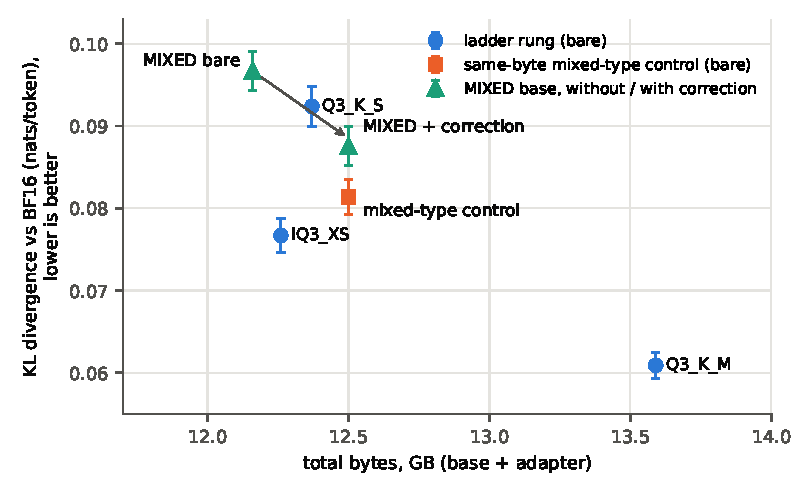
\includegraphics[width=0.88\linewidth]{figures/fig-ladder-27b.pdf}
\small\caption{Qwen3.6-27B near 12.5 GB, 100 chunks, every file one quantization step from BF16; error bars are standard errors. The correction (arrow) moves the mixed base past the stock type Q3\_K\_S; a mixed-type control with no adapter at the same bytes is lower, and the I-quant type IQ3\_XS is the lowest of the group.}
\end{figure}

\textbf{0.6B and 0.8B.} At 0.6B the corrected configuration (two alternation rounds, full-covariance correction, Q8\_0 factors; 382 MB) reaches perplexity 25.27 and KLD 0.209 against Q3\_K\_M at 347 MB (26.06 and 0.238); the KLD difference is about 5 unpaired standard errors, on-distribution\src{rollup, review}. At 0.8B, scored against BF16, a rank-128 full-covariance correction of Q2\_K ties Q3\_K\_M, and one alternation round is ahead of it at 9\% more bytes (KLD 0.147 against 0.167; no error bars were logged for this row)\src{E22}.

At both sizes the comparison rung was chosen from below. Linear interpolation between the neighbouring rungs at the corrected configuration’s byte count (about 0.118 at 382 MB and 0.080 at 523 MB) is better than the corrected configuration, and Q4\_K\_M at 4\% more bytes is three to four times lower in KLD. A stock rung scored later against the same 0.8B reference, Q4\_K\_S at 519 MB, has KLD 0.047 against the 523 MB corrected configuration’s 0.147 (unpaired)\src{E34}. No mixed-type control was built at these sizes. What the small-scale runs show is that the method transfers to a second architecture and lands between two discrete rungs; they do not show a result against the ladder.

A correction on an NVFP4 base at 0.8B improves its base and loses to every stock rung at or below its bytes; the details are in Appendix A.1.

\textbf{Two qualifications on all of the above.} Every corrected configuration pays a decode cost of 20-40\% on stock llama.cpp that the bare rungs do not (\hyperref[sec:6]{§6}). And the tables in this subsection are on-distribution: calibration and evaluation share wikitext-2 (train and test splits), and \hyperref[sec:4.8]{§4.8} shows the method is sensitive to distribution. The held-out evidence for the correction increment at 27B is the FineWeb-Edu control of \hyperref[sec:5.3]{§5.3}; the ladder comparisons themselves have not been repeated on a held-out corpus.

\subsection*{\phantomsection\label{sec:4.4}4.4\hspace{0.8em}Three placements of the low-rank bytes, and a bound on their difference}
\addcontentsline{toc}{subsection}{4.4 Three placements of the low-rank bytes, and a bound on their difference}

A set of pre-registered paired experiments at 27B asked whether it matters where the low-rank bytes act. Three placements were built at matched bytes on the mixed base. The first is the post-hoc correction of \hyperref[sec:2.2]{§2.2}. The second is a pre-quantization carve in the preserve-then-quantize order (\cite{arxiv2602.02001}): take a whitened rank-128 component C = B·A off the BF16 weights, quantize the remainder with the same mixed recipe, and serve C as the adapter. The third shares one A factor across tensors that read the same input (the arrangement of \cite{arxiv2603.25385}), in two variants: at byte parity with the first placement, and at rank 128.

Their surrogate scores differ. The post-hoc correction captures 0.42 of the whitened residual. The carve captures 76\% of the whitened weight matrix at rank 128 on a 12-tensor sample. The shared basis at byte parity captures 12.2\% more whitened energy than separate bases on the attention groups and 6.9\% more on the GDN groups; at equal rank it keeps 99.55\% and 99.75\% of the separate capture\src{E28, E29}.

Their measured quality does not. Each alternative placement minus the post-hoc correction, on 100 paired chunks\src{E35}:

\begin{center}\fontsize{8.5}{10.5}\selectfont\setlength{\tabcolsep}{4pt}
\begin{tabularx}{\linewidth}{@{}llll>{\hsize=1.000\hsize\raggedright\arraybackslash}X@{}}
\toprule
\textbf{placement vs post-hoc correction} & \textbf{ΔKLD} & \textbf{t} & \textbf{90\% interval} & \textbf{largest bound as a share of the correction’s increment (0.0090)} \\
\midrule
pre-quantization carve & +0.0017 ± 0.0017 & +0.99 & {}[−0.0011, +0.0045] & 49\% \\
shared basis, byte parity & −0.0005 ± 0.0006 & −0.91 & {}[−0.0015, +0.0004] & 17\% \\
shared basis, rank 128 & −0.0008 ± 0.0006 & −1.48 & {}[−0.0018, +0.0001] & 20\% \\
\bottomrule
\end{tabularx}
\end{center}

Three low-rank placements differ by less than 0.0045 KLD (90\% interval), under 50\% of the correction’s own increment (0.0090); for the two shared-basis variants the bound is 0.0018, about 20\%. We could not distinguish them. This is a bound and not a demonstration that the placements are the same: the interval for the carve admits a deficit of half an increment, its top-1 difference leans negative (t = −1.68), and it trails the control by more than the others do. One mixed-type control at the same bytes is better than all four files (t = +2.62, +5.15, +2.35 and +2.39 for the post-hoc correction, the carve, and the two shared-basis variants).

Scope: one model, one byte count, one rank, one corpus, with three arms that share a base recipe and a Gram. The statement that type allocation does better rests on one designed control. Per-tensor type allocation is the axis that RCO (\cite{arxiv2605.00649}) optimizes under an exact byte budget; that paper does not compare placements, and this one does not optimize allocation.

A related family uses seeded, unlearned bases (AWSRC, \cite{arxiv2608.23144}). A pre-registered capture comparison on our cached whitened spectra (18 tensors, 3 seeds) finds that such bases capture 0.035 of the dominant whitened energy at byte parity against 0.983 for learned factors, which is the random-subspace expectation\src{E31}. We did not run a quality comparison for that family.

One by-product: the shared basis at rank 128 is within the bound above of the post-hoc correction while storing fewer distinct factor bytes. If a loader aliased the shared factor, the adapter would occupy 280.8 MB against 336.5 MB (−16.6\%). That figure is a computed size under a loader patch we did not write; the file that was evaluated stores the duplicates and is 336.5 MB\src{E28}.

\subsection*{\phantomsection\label{sec:4.5}4.5\hspace{0.8em}Recovery grows as the base gets thinner, and factors do not replace base bits}
\addcontentsline{toc}{subsection}{4.5 Recovery grows as the base gets thinner, and factors do not replace base bits}

With the estimator held to full covariance, the fraction of the base’s KLD damage that correction recovers rises as the base gets thinner: 20\% at Q2\_K, 28\% at IQ2\_XS, 41\% at IQ1\_S (legacy 27B rows)\src{rollup, review}. The three points do not hold the recipe fixed: adapter budgets are 0.93, 0.93 and 0.80 GB and the rank mix varies, so the curve is confounded. Its direction agrees with the published claim that correction pays most at the lowest bit widths (\cite{arxiv2604.07955}) and with EoRA’s results.

Pushing this to the thinnest base llama.cpp offers, IQ1\_S with 2.52 GB of factors, still loses to bare Q2\_K at near-equal total bytes by about a factor of three in KLD. Per gigabyte, added factor bytes bought about 0.06 KLD where base bits bought 0.22 to 0.32. The details are in Appendix A.2.

\subsection*{\phantomsection\label{sec:4.6}4.6\hspace{0.8em}Mixture-of-experts: correction loses to a one-line promotion (n = 20, Q4-referenced)}
\addcontentsline{toc}{subsection}{4.6 Mixture-of-experts: correction loses to a one-line promotion (n = 20, Q4-referenced)}

On Qwen3.6-35B-A3B (256 experts per stack, 8 routed; expert stacks are 91\% of parameters) both correction variants improve their base and both lose to the ladder, with a control built from the start\src{E23}. Two limits apply to every number in this subsection: n = 20 chunks, and the reference is not BF16. We had no BF16 of this model, so every file is one quantization step from the vendor UD-Q4\_K\_M file (22.1 GB) and KLD is measured against that file’s logits.

Per-expert whitened correction (rank 32, Q8\_0 factors, pooled-Gram whitening; served on stock llama.cpp, which handles three-dimensional adapter pairs) improves the Q2\_K base (t = −4.55, 18/20 chunks); a shared-basis variant improves it weakly (t = −2.69, 13/20). At its byte count (14.5 GB) the per-expert correction loses to a control that promotes ffn\_down\_exps to Q4\_K, by +0.0257 ± 0.0038 KLD (t = +6.85, 0/20 chunks), and the shared-basis variant loses to the same control at t = +9.33. Q3\_K\_S, 0.7 GB larger than the corrected file, is lower again (KLD 0.1150 against the control’s 0.1666; control versus Q3\_K\_S, t = +8.15). Per byte added to the base, the promotion control removes 2.6 times as much KLD as the rank-32 factors, and Q3\_K\_S 4.2 times as much\src{E35}.

Because the control promotes a tensor group toward the reference’s own bit width, we checked whether the reference favours it by construction. In the vendor reference, ffn\_down\_exps is Q5\_K in 37 layers and Q6\_K in 3 (from the quantize log and from the GGUF header); the up and gate stacks are Q4\_K. The control’s Q4\_K is therefore a real quantization step below the reference and not a copy of it. The comparison still measures distance to a quantized model and should be repeated against BF16 when one is available\src{E35}.

The structural result is about sharing. One output basis per stack, shared by 256 experts, captures 0.086-0.090 of whitened residual energy on the up and gate stacks against 0.0625 for a random orthonormal basis, and 0.022 against 0.0156 on the down stacks. The pooled whitened residual is nearly isotropic, so there is no common subspace to amortize at rank 32. Each expert is a 512 × 2,048 matrix whose residual is weakly structured (per-expert capture 0.19-0.36, measured under the pooled whitener, which approximates each expert’s own input covariance), and the factor overhead is paid 256 times. Correcting the dense tensors of a mixture-of-experts model, or expert bases below 2 bits where no cheap promotion exists, were not tried.

\subsection*{\phantomsection\label{sec:4.7}4.7\hspace{0.8em}When a better surrogate did not give a better outcome}
\addcontentsline{toc}{subsection}{4.7 When a better surrogate did not give a better outcome}

Metric quality mattered more than rank. Going from diagonal to full-covariance whitening at 0.6B was worth more than doubling rank: full covariance at rank 64 gives perplexity 27.58 and KLD 0.318, against 31.29 and 0.420 for the diagonal at rank 64 and 28.46 for the diagonal at rank 128 (about 10 and 2.6 unpaired standard errors). The same comparison at 27B was about 2 unpaired standard errors (0.1460 → 0.1282 at rank 64)\src{E10}.

In the other direction, improving a surrogate repeatedly failed to improve the outcome.

Rank allocation by greedy energy water-filling at 0.6B is worse than uniform rank at equal bytes (perplexity 34.17 against 31.29); it assigns no rank to ffn\_down. Measured per-kind KL sensitivities give a different ordering (attn\_k highest at 0.0128 ΔKLD per MB; isolated sensitivities sum to 0.352 against a joint 0.346). The end-to-end margin of allocated over uniform rank at 27B is unresolved (0.5 unpaired standard errors), and the 27B weights were priors carried over from 0.6B\src{journal, review}.

Sensitivity estimated from one side anti-correlates with measured sensitivity (Spearman −0.29 for the gradient side, as for the input side); the two-sided product correlates positively (+0.39)\src{E20}. Measured two-sided full-covariance correction at 0.6B gives 27.27 against 27.58 one-sided at equal bytes.

The full list, with the cases reported in other sections:

\begin{center}\fontsize{8.5}{10.5}\selectfont\setlength{\tabcolsep}{4pt}
\begin{tabularx}{\linewidth}{@{}l>{\hsize=0.913\hsize\raggedright\arraybackslash}X>{\hsize=1.087\hsize\raggedright\arraybackslash}Xl@{}}
\toprule
\textbf{\#} & \textbf{what improved on the surrogate} & \textbf{what the outcome did} & \textbf{where} \\
\midrule
1 & energy captured by greedy rank allocation & perplexity worse than uniform (34.17 vs 31.29) & this section \\
2 & exact descent of a two-sided Kronecker metric with measured T & +0.048 nats vs input-only (t = +15.5); worse than the untouched file with a cleaner T & \hyperref[sec:3.2]{§3.2} \\
3 & a further 2.6\% descent of the same whitened objective & no change (|t| ≤ 1.32) & Appendix A.4 \\
4 & importance moved into column scales (equalization) & perplexity 33.09 → 41.73 (t = +28 on KLD, +60 on NLL) & Appendix A.3 \\
5 & whitened capture at equal bytes (shared basis, +12\% on attention groups) & KLD within the bound of \hyperref[sec:4.4]{§4.4} (t = −0.91) & \hyperref[sec:4.4]{§4.4} \\
6 & residual capture of the base (NVFP4 0.736 vs Q3\_K\_M 0.721) & smaller gain (50\% vs 70\% recovery) & Appendix A.1 \\
7 & 512-token KL divergence, across refinement families & opposite ordering on a coding suite; one pair, one run per arm, unreplicated & \hyperref[sec:5.5]{§5.5} \\
\bottomrule
\end{tabularx}
\end{center}

Rows 1-6 are surrogates for KL divergence that did not predict KL divergence. Row 7 is of a different kind and weaker: KL divergence against a task outcome, in a single pair. We do not have evidence that KL divergence predicts task outcomes at the size of the contested margins within a family either: the one task evaluation we ran there (HellaSwag, \hyperref[sec:4.3]{§4.3}) tied the contested pair.

\subsection*{\phantomsection\label{sec:4.8}4.8\hspace{0.8em}Conditioning the correction on a task distribution}
\addcontentsline{toc}{subsection}{4.8 Conditioning the correction on a task distribution}

Conditioning the correction’s covariance on a code corpus gives 10.3\% lower perplexity on code at identical bytes (2.746 against 3.061 for the wikitext-conditioned correction; about 8 unpaired standard errors) and costs 27\% on wikitext (34.90 against 27.58). Broad calibration transfers to a narrow distribution better than the reverse\src{E17}. Per-workload adapters are possible through llama.cpp’s per-request adapter API. The same measurement is a caution: the method’s sensitivity to distribution (10-27\%) is larger than every contested margin in \hyperref[sec:4.3]{§4.3}, which is why \hyperref[sec:3.1]{§3.1} and \hyperref[sec:5.3]{§5.3} report held-out corpora and why the comparisons of \hyperref[sec:4.3]{§4.3} are labeled on-distribution.

\subsection*{\phantomsection\label{sec:4.9}4.9\hspace{0.8em}Ordering of operations}
\addcontentsline{toc}{subsection}{4.9 Ordering of operations}

From \hyperref[sec:3.3]{§3.3} and the alternation runs: shaping the base and the corrector jointly beats composing them greedily. At 0.6B, two alternation rounds (perplexity 25.27) are better than a one-shot re-round under a ProjQ-style metric (25.94), which is better than re-round-then-correct (26.80); these are unpaired, and the ordering is paired-resolved at 0.8B (\hyperref[sec:3.3]{§3.3})\src{E13, review}. The alternation is LoftQ’s; what is specific here is the black-box llama-quantize grid and the whitened metric. A second rule comes from the mixed base and from \hyperref[sec:4.5]{§4.5} and \hyperref[sec:4.6]{§4.6}: put the correction where rank is a large fraction of width, and spend base bits elsewhere.

\section*{\phantomsection\label{sec:5}5\hspace{0.8em}A head-to-head with released trained checkpoints}
\addcontentsline{toc}{section}{5. A head-to-head with released trained checkpoints}

\subsection*{\phantomsection\label{sec:5.1}5.1\hspace{0.8em}Setup, bytes and cost}
\addcontentsline{toc}{subsection}{5.1 Setup, bytes and cost}

GSQ-RCO (\cite{arxiv2604.18556}, \cite{arxiv2605.00649}) is released as refined GGUF checkpoints of Qwen3.8-27B. By its model card, every tensor is quantized with GSQ (Gumbel-Softmax re-selection of codes) at every candidate GGUF type, RCO selects one type per tensor under an exact byte budget, and the selections are assembled into a standard GGUF. The public GSQ repository contains no GGUF path, so we compare the released files and make no statement about the mechanism that produced them. The comparison was pre-registered on the Unsloth Dynamic baselines the card compares against, scored on 40 chunks of wikitext-2 test against BF16 reference logits, with a fresh 48-chunk BF16 imatrix and Gram capture\src{E32}.

The three arms are not byte-matched, and every statement below should be read against this table:

\begin{center}\fontsize{8.5}{10.5}\selectfont\setlength{\tabcolsep}{4pt}
\begin{tabular}{@{}lll@{}}
\toprule
\textbf{arm} & \textbf{IQ2 class} & \textbf{IQ3 class} \\
\midrule
GSQ-RCO, trained & IQ2\_XS, 8.42 GB & IQ3\_S, 11.77 GB \\
Unsloth baseline, untrained & UD-IQ2\_S, 8.37 GB & UD-IQ3\_S, 12.04 GB \\
baseline plus our correction & 9.27 GB (8.37 + 0.90 adapter) & 12.94 GB (12.04 + 0.90 adapter) \\
stock file near the corrected arm’s bytes & UD-Q2\_K\_XL, 9.83 GB & none measured \\
\bottomrule
\end{tabular}
\end{center}

Our arm is a rank-128 full-covariance correction with Q8\_0 factors on the Unsloth baseline. It is larger than the GSQ-RCO file by 0.85 GB in the IQ2 class and by 1.17 GB in the IQ3 class. The re-rounder was not used, because its codec does not cover the I-quant formats.

The cost of our arm, end to end: the extraction takes about 12 CPU-minutes per model (724, 727 and 744 seconds). That figure excludes obtaining the BF16 weights (54.7 GB) and the 48-chunk Gram capture, which needs our patched build and which the capture log estimated at about 22 minutes. The released checkpoints come from a GPU training run whose cost we did not measure\src{E32}.

\subsection*{\phantomsection\label{sec:5.2}5.2\hspace{0.8em}512-token KL divergence on wikitext}
\addcontentsline{toc}{subsection}{5.2 512-token KL divergence on wikitext}

Paired per-chunk differences, wikitext-2 test, n = 40\src{E32, E35}:

\begin{center}\fontsize{8.5}{10.5}\selectfont\setlength{\tabcolsep}{4pt}
\begin{tabular}{@{}lllll@{}}
\toprule
\textbf{pair (A − B)} & \textbf{ΔKLD} & \textbf{t} & \textbf{A better on} & \textbf{Wilcoxon p} \\
\midrule
GSQ-RCO IQ2\_XS vs UD-IQ2\_S (8.42 vs 8.37 GB) & +0.0715 ± 0.0061 & +11.68 & 0/40 & 2e-12 \\
GSQ-RCO IQ3\_S vs UD-IQ3\_S (11.77 vs 12.04 GB) & +0.0152 ± 0.0018 & +8.56 & 1/40 & 6e-11 \\
corrected vs own base, IQ2\_S (+0.90 GB) & −0.0122 ± 0.0019 & −6.45 & 39/40 & 9e-12 \\
corrected vs own base, Q2\_K\_XL (+0.90 GB) & −0.0055 ± 0.0008 & −6.98 & 34/40 & 2e-8 \\
corrected vs own base, IQ3\_S (+0.90 GB) & −0.0021 ± 0.0004 & −5.89 & 36/40 & 1e-6 \\
corrected IQ2\_S vs GSQ-RCO IQ2\_XS (9.27 vs 8.42 GB) & −0.0837 ± 0.0073 & −11.49 & 40/40 & 2e-12 \\
corrected IQ3\_S vs GSQ-RCO IQ3\_S (12.94 vs 11.77 GB) & −0.0173 ± 0.0018 & −9.48 & 38/40 & 9e-12 \\
corrected IQ2\_S vs UD-Q2\_K\_XL (9.27 vs 9.83 GB) & +0.0337 ± 0.0029 & +11.59 & 0/40 & 2e-12 \\
\bottomrule
\end{tabular}
\end{center}

Three readings, in order of byte fairness. First, at matched bytes the untrained vendor baseline already has lower KLD than the trained checkpoint at both classes (rows 1-2). Second, our correction lowers its own base at all three rungs, at a cost of 0.90 GB (rows 3-5); top-1 agreement rises at the two 2-bit rungs (+0.7 points, t about +3.8) and not at IQ3\_S (t = +0.5). Third, the gap between the corrected arm and GSQ-RCO (rows 6-7) is mostly the first effect: at the IQ2 class, 0.0715 of the 0.0837 (85\%) is the baseline’s lead and 0.0122 (15\%) is the correction; at the IQ3 class, 0.0152 of 0.0173 (88\%) and 0.0021 (12\%).

Against the ladder the result is that of \hyperref[sec:4.3]{§4.3}. The stock UD-Q2\_K\_XL file at 9.83 GB is better than the corrected IQ2\_S arm at 9.27 GB by 0.0337 KLD (row 8). The two are 0.56 GB apart, so this is a near-equal-byte comparison and not an equal-byte one.

\begin{figure}[!htbp]\centering
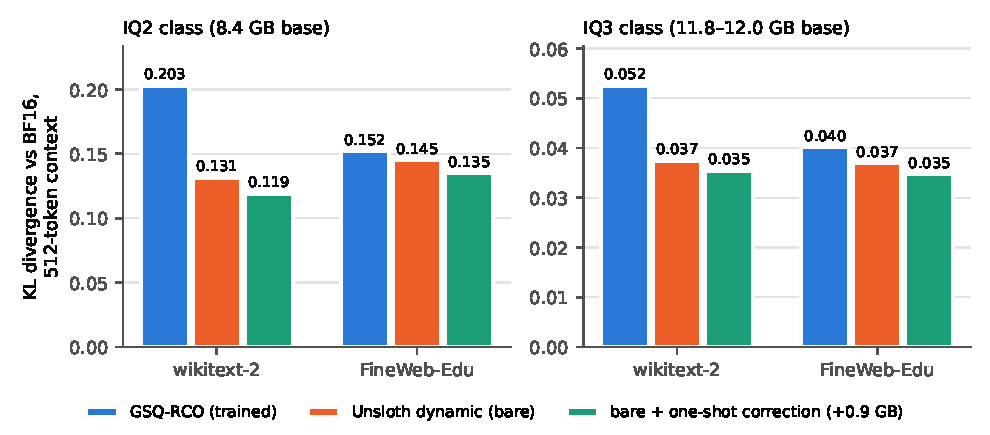
\includegraphics[width=0.88\linewidth]{figures/fig-gsq-kld.pdf}
\small\caption{Released GSQ-RCO checkpoints of Qwen3.8-27B against their untrained Unsloth baselines and against the baseline plus a one-shot whitened correction, on two corpora (40 chunks each). The corrected arm carries a 0.9 GB adapter and is not byte-matched to the other two.}
\end{figure}

\subsection*{\phantomsection\label{sec:5.3}5.3\hspace{0.8em}A second corpus, and both halves of a registered prediction}
\addcontentsline{toc}{subsection}{5.3 A second corpus, and both halves of a registered prediction}

The wikitext result admits a calibration-mismatch reading: the released files may be tuned to text unlike wikitext. The calibration corpus of the released files is not documented. An earlier entry in our journal said they were trained on FineWeb-Edu; a check of the card and the released code the next day found no support for that, and the control was registered with the corrected wording: FineWeb-Edu is used because it is the one non-wikitext corpus the card reports on\src{journal}.

The registration made a two-part prediction for the mismatch reading: the GSQ-RCO deficit against its baseline would shrink materially or change sign on FineWeb-Edu, and our own increments, whitened by wikitext Grams, would shrink too. The alternative reading predicted a GSQ-RCO deficit of t \ensuremath{\gtrsim} +4. The same eight contrasts on 40 chunks of FineWeb-Edu, against a BF16 reference on that text\src{E32, E35}:

\begin{center}\fontsize{8.5}{10.5}\selectfont\setlength{\tabcolsep}{4pt}
\begin{tabular}{@{}lllll@{}}
\toprule
\textbf{pair (A − B), FineWeb-Edu, n = 40} & \textbf{ΔKLD} & \textbf{t} & \textbf{A better on} & \textbf{Wilcoxon p} \\
\midrule
GSQ-RCO IQ2\_XS vs UD-IQ2\_S & +0.0073 ± 0.0044 & +1.66 & 13/40 & 0.022 \\
GSQ-RCO IQ3\_S vs UD-IQ3\_S & +0.0033 ± 0.0016 & +2.07 & 13/40 & 0.029 \\
corrected vs own base, IQ2\_S & −0.0103 ± 0.0011 & −9.40 & 38/40 & 1e-11 \\
corrected vs own base, Q2\_K\_XL & −0.0052 ± 0.0006 & −9.20 & 38/40 & 5e-8 \\
corrected vs own base, IQ3\_S & −0.0022 ± 0.0003 & −8.65 & 36/40 & 1e-7 \\
corrected IQ2\_S vs GSQ-RCO IQ2\_XS & −0.0175 ± 0.0045 & −3.94 & 35/40 & 1e-4 \\
corrected IQ3\_S vs GSQ-RCO IQ3\_S & −0.0055 ± 0.0016 & −3.39 & 31/40 & 3e-4 \\
corrected IQ2\_S vs UD-Q2\_K\_XL & +0.0471 ± 0.0044 & +10.72 & 1/40 & 4e-12 \\
\bottomrule
\end{tabular}
\end{center}

The first half of the prediction held. The GSQ-RCO deficit falls about tenfold at the IQ2 class (+0.0715 to +0.0073) and fivefold at the IQ3 class (+0.0152 to +0.0033), to a difference that is unresolved by t at IQ2 and marginal at IQ3. On FineWeb-Edu the matched-byte comparison of trained checkpoint and untrained baseline is close to a tie.

The second half mostly did not hold. Our increments were predicted to shrink; the IQ2\_S increment is 16\% smaller (−0.0122 to −0.0103) and the other two are unchanged (−0.0055 to −0.0052; −0.0021 to −0.0022). The registered mismatch reading is therefore supported for the competitor’s arm and not for ours, and we report it as a prediction that was half wrong. The useful consequence is a held-out measurement of the correction increment at 27B: a correction whitened on wikitext lowers its base on FineWeb-Edu by nearly the same amount.

With the baseline and the trained checkpoint close on this corpus, the corrected arm’s lead over GSQ-RCO (−0.0175 and −0.0055) is about the size of the correction increment, which is bought with 0.9 GB. The stock UD-Q2\_K\_XL file again beats the corrected IQ2\_S arm at near-equal bytes.

\subsection*{\phantomsection\label{sec:5.4}5.4\hspace{0.8em}Perplexity at two context lengths}
\addcontentsline{toc}{subsection}{5.4 Perplexity at two context lengths}

The card’s wikitext perplexities order GSQ-RCO ahead of the Unsloth baseline at both classes. At our 512-token context the means order them the other way, and the paired difference is unresolved: ΔNLL (GSQ-RCO minus baseline) +0.017 ± 0.013 (t = +1.33) at the IQ2 class and +0.003 ± 0.006 (t = +0.58) at the IQ3 class, n = 40.

At a 2048-token context the card’s ordering reproduces: GSQ-RCO IQ2\_XS 6.834 ± 0.043 against UD-IQ2\_S 7.119 ± 0.047, and GSQ-RCO IQ3\_S 6.306 ± 0.039 against UD-IQ3\_S 6.417 ± 0.041\src{E32}. Paired over the 145 chunks, the NLL difference is −0.041 ± 0.012 (t = −3.33) at the IQ2 class and −0.018 ± 0.004 (t = −4.15) at the IQ3 class. The IQ3 result is consistent across tests (GSQ-RCO ahead on 89/145 chunks, Wilcoxon p = 1e-4). The IQ2 result is carried by a minority of chunks: GSQ-RCO is ahead on 77/145 (sign test p = 0.51, Wilcoxon p = 0.035)\src{E35}.

So the 512-token perplexity ordering is unresolved and the 2048-token ordering is resolved in the checkpoint’s favour. We did not measure KL divergence at 2048 tokens, so this experiment does not separate the effect of context length from the difference between perplexity and KL divergence. Every KL-divergence number in this paper is at 512 tokens.

\subsection*{\phantomsection\label{sec:5.5}5.5\hspace{0.8em}One capability pair}
\addcontentsline{toc}{subsection}{5.5 One capability pair}

The card’s claims are task-level. We ran the 112-unit fast subset of an agentic coding suite (multi-language tasks solved by an agent loop with a compiler and tests; single-slot serving, stock llama.cpp b10865, reasoning budget capped at 20,480 tokens) on the two IQ3-class files, once each\src{E32}:

\begin{center}\fontsize{8.5}{10.5}\selectfont\setlength{\tabcolsep}{4pt}
\begin{tabularx}{\linewidth}{@{}>{\hsize=1.000\hsize\raggedright\arraybackslash}Xlll@{}}
\toprule
\textbf{file} & \textbf{passed (of 112)} & \textbf{of which Zig (of 30)} & \textbf{completion tokens} \\
\midrule
GSQ-RCO IQ3\_S & 88 & 9 & 2.40 M \\
Unsloth UD-IQ3\_S & 76 & 2 & 2.75 M \\
for scale: a different finetune of the same model at Q5\_K\_M, four runs & 82, 84, 85, 91 & not tabulated & not tabulated \\
\bottomrule
\end{tabularx}
\end{center}

Paired by unit, 16 units pass only under GSQ-RCO and 4 only under the baseline, a net of +12 (exact McNemar p = 0.012). Five things limit what this supports.

\begin{itemize}
\item\relax It is one run per arm.
\item\relax The four-run band is from a different finetune, so a file landing inside it is not evidence that the file is lossless. What the band does show is a 9-unit run-to-run spread for one unchanged file, against which a +12 difference between two single runs has to be read.
\item\relax Seven of the twelve come from Zig, where both arms are near the floor (9/30 and 2/30); the direction is the same in Zig (+7, p = 0.065) and elsewhere (+5, p = 0.18), and neither part is resolved alone.
\item\relax McNemar’s test treats each unit’s outcome as deterministic, which the band’s spread contradicts.
\item\relax The record does not state whether the band runs used the same single-slot serving configuration.
\end{itemize}

A first attempt at these rows under six-slot serving was retracted after both IQ3-class files crashed the server. The IQ2 capability pair was started and not completed, and our corrected arm was not run on the suite.

\subsection*{\phantomsection\label{sec:5.6}5.6\hspace{0.8em}What the head-to-head shows}
\addcontentsline{toc}{subsection}{5.6 What the head-to-head shows}

Against released GSQ-RCO checkpoints, the untrained vendor baseline at matched bytes already has lower 512-token KLD on wikitext (not resolved on FineWeb-Edu); adding our correction (+0.9 GB, not byte-matched) lowers it further on both corpora. A stock rung at near-equal total bytes beats the corrected arm. In one cross-family pair (one run per arm), 512-token KLD and a coding suite ordered the artifacts oppositely; we treat 512-token KLD as unvalidated across refinement families. On FineWeb-Edu the KLD difference in that pair is close to a tie, so there the disagreement is a tie against a single-run win. We have no task measurement of our own arm and make no claim that the corrected file is the more capable one.

\section*{\phantomsection\label{sec:6}6\hspace{0.8em}Serving: the adapter’s decode cost and how much of it kernels remove}
\addcontentsline{toc}{section}{6. Serving: the adapter's decode cost and how much of it kernels remove}

\subsection*{\phantomsection\label{sec:6.1}6.1\hspace{0.8em}The cost on stock llama.cpp}
\addcontentsline{toc}{subsection}{6.1 The cost on stock llama.cpp}

Every corrected configuration in \hyperref[sec:4]{§4} and \hyperref[sec:5]{§5} carries a decode cost that a bare quantized file does not. On stock llama.cpp the adapter path adds two unfused matrix-vector launches per projection. At batch 1 this costs 33-39\% of decode speed at 0.6B (667 → 444 and 407 tok/s). At 27B it costs 33\% with F16 rank-64 factors (99.7 → 66.5 tok/s) and 19\% with Q8\_0 factors (99.7 → 81.0)\src{rollup, E35}. Others report the same pattern: adapter operations at batch 1 are bound by launches and not by rank (\cite{arxiv2310.18547}; \cite{arxiv2603.11873}; \cite{arxiv2605.08314}; CALDERA’s Table 6, \cite{arxiv2405.18886}). A corrected configuration that is competitive with a rung on bytes is therefore not competitive with it on stock llama.cpp today.

The kernels below remove most of that cost on local, unmerged patches. They leave perplexity digit-identical and each has a switch to disable it. All speed comparisons are same-session A/B pairs, because drift between sessions on identical configurations reached 9\% and invalidated one number in our first tables (86.3 tok/s, 82.3 on re-measurement)\src{review}.

\textbf{Evidence grade.} Only one speed result in this section has raw benchmark output in the repository: the N = 10 interleaved pair at 27B (\hyperref[sec:6.2]{§6.2}). Every other speed number is transcribed from the per-phase reports, which record the measurements as prose tables. All of them come from one GPU and one host, at a pinned build (llama.cpp 0ef6e55ed). The patch set has since been rebased onto b10865 and no speed number was re-measured after the rebase.

\subsection*{\phantomsection\label{sec:6.2}6.2\hspace{0.8em}Three phases of kernel fusion}
\addcontentsline{toc}{subsection}{6.2 Three phases of kernel fusion}

\textbf{Window fusion.} The five-node subgraph llama.cpp emits per adapted projection (W·x, A·x, B·t, scale, add) is matched in the CUDA backend and collapsed to two kernels. The result was +10\% at rank 16 and no change at rank 64: removing 588 of 784 extra kernel launches per token did not move rank-64 decode, so launch count was not the bottleneck on an idle GPU\src{E14}.

\textbf{Folding A into the activation-quantize kernel.} Following the design of SVDQuant (\cite{arxiv2411.05007}), we fold t = A·x into the existing activation-quantize launch and B·t into the matrix-vector epilogue. Rank-64 decode at 0.6B went from 476 to 685 tok/s (+44\%), which reduced the adapter cost in that session from 45\% to 20\%. The constant cost had been serialization: the epilogue loaded B and t after the main dot-product loop, adding a memory-latency round to every kernel. Loading static operands before the grid-dependency synchronization point removes it\src{E14}.

\textbf{Quantized factors and register pressure.} Accepting Q8\_0 factors in the fused paths gave +62\% at 0.6B (394 → 638) and at first slowed 27B by 6.6\%, because unfused Q8\_0 factors already use an int8 kernel upstream. Two size gates restored +0.4\% at 27B\src{E14}. The remaining 27B cost was register pressure: the fused kernel carried about 19 extra registers (61 → 80), which lowered occupancy. Moving the adapter dot product ahead of the main loop, with its result held in shared memory, restored 62 registers. Same-session pairs after that change: 0.6B 391 → 702 tok/s (+79\%, one pair); 27B 84.7 → 86.9 (+2.6\%, one pair)\src{E14}.

Re-measured on a quiet host with interleaved blocks (N = 10, median and interquartile range), the 27B corrected configuration decodes at 88.1 [88.0-88.3] tok/s fused against 85.8 [85.7-85.8] unfused: +2.7\%, against a measured ceiling of +4.9\% for any epilogue design\src{E27}.

Two practices came out of this that may transfer to other memory-bound matrix-vector kernels: load static operands before the grid-dependency synchronization, and keep the epilogue from adding registers to the main loop by holding its state in shared memory.

\subsection*{\phantomsection\label{sec:6.3}6.3\hspace{0.8em}An allocator fix for stream concurrency}
\addcontentsline{toc}{subsection}{6.3 An allocator fix for stream concurrency}

llama.cpp’s CUDA graph optimization was rejecting stream concurrency on adapter graphs, correctly: the allocator keeps one global free list, so a buffer freed in one branch of a fork can be handed to a tensor in a concurrent branch. Our change pins buffers within a fork-join region: frees inside a region are deferred to the join, and an in-place guard keeps the last consumer of a forked tensor from taking a buffer another stream still reads. The backend test suite (12,996 cases) passes, perplexity is digit-identical, and 200-token greedy generation is string-identical with the change on and off on three configurations.

The speed result is modest and was measured on a loaded host (load 40-66 on 32 threads throughout). At 0.6B, base-model decode rose in two sessions by 11\% (763 → 849 tok/s) and by 19.6\% (794 → 950); the report calls the second the best pair. With an adapter the gain was 7-12\%. At 27B, six alternated sessions showed no difference outside noise: streams cover only the one-in-four full-attention layers of the hybrid architecture, and the large matrix-vector products already fill the GPU\src{E25}. The change does not depend on adapters.

\subsection*{\phantomsection\label{sec:6.4}6.4\hspace{0.8em}Where the decode cost stands}
\addcontentsline{toc}{subsection}{6.4 Where the decode cost stands}

At 0.6B the adapter cost on the patched build is about 20\%, down from 45\%. At 27B the fused corrected configuration (88.1 tok/s) is within the +4.9\% ceiling of the unfused one, so with Q8\_0 factors little of the remaining cost is in the epilogue. What remains against a bare rung is the adapter’s VRAM and the per-token chain of extra nodes, which published work prices at 1.3-2 µs per node (\cite{arxiv2512.22219}). None of the patches is merged upstream.

\section*{\phantomsection\label{sec:7}7\hspace{0.8em}Limitations and open work}
\addcontentsline{toc}{section}{7. Limitations and open work}

\subsection*{\phantomsection\label{sec:7.1}7.1\hspace{0.8em}Limitations}
\addcontentsline{toc}{subsection}{7.1 Limitations}

\textbf{Models and hardware.} Every model is Qwen-family: Qwen3-0.6B, Qwen3.5-0.8B, Qwen3.6-27B (as the heretic-v2 finetune), Qwen3.8-27B and Qwen3.6-35B-A3B. Every measurement comes from one GPU (an RTX 5090) on one workstation. Nothing here tests another model family.

\textbf{Baselines not compared.} The re-rounder was compared against the file it starts from and, at 0.8B, against stock rungs. It was never compared against free-grid GPTQ at equal bits, against vector or lattice quantizers at 2 bits, or against learned-rounding methods. The type-allocation control was built by hand from measured sensitivities and was not compared against Hessian-aware mixed-precision allocation methods. These are named as classes of work; we did not run them and do not cite numbers for them.

\textbf{Distribution.} Calibration and most evaluation share wikitext-2 (train and test splits). The corrected configurations carry more calibration-fitted capacity than the rungs they are compared with, and \hyperref[sec:4.8]{§4.8} measures 10-27\% sensitivity to the corpus, larger than every contested ladder margin. Off-distribution we have: the re-rounder at 0.8B on a code corpus and on an unseen prose corpus (\hyperref[sec:3.1]{§3.1}), and the correction increment at 27B on FineWeb-Edu (\hyperref[sec:5.3]{§5.3}). The ladder comparisons of \hyperref[sec:4.3]{§4.3} have not been repeated on a held-out corpus, and neither has the 27B re-rounder.

\textbf{Statistics.} The t statistics are conditional on one calibration sample and one evaluation corpus. No family-wise correction was applied. The two contested 27B margins are a third look at accumulating data, one of them is not uniform across the test set, and neither is replicated (\hyperref[sec:4.3]{§4.3}). Blocks in the block bootstrap are runs of consecutive chunks and not articles.

\textbf{The instrument.} Every KL-divergence number is at a 512-token context. In one pair of files it ordered them opposite to a coding suite (\hyperref[sec:5.5]{§5.5}), and the only task evaluation inside our own comparisons tied the contested pair (\hyperref[sec:4.3]{§4.3}). Task-level evidence in this paper is thin: one multiple-choice benchmark at one byte count, and one coding suite, one run per arm, on the competitor’s files only. None of our corrected or re-rounded files was run on the coding suite.

\textbf{Controls.} The mixed-type control exists at 27B and for the mixture-of-experts model. It was not built at 0.6B or 0.8B, and it is a single designed point at each size where it exists.

\textbf{Width.} The regression of \hyperref[sec:4.2]{§4.2} has one step on the width axis and its intervals resample tensors, not models.

\textbf{References and precision.} Rows labeled legacy are scored against a Q6\_K or Q8\_0 file and not BF16 (measured contamination at 27B: 0.0032 KLD). The mixture-of-experts table is scored against a vendor Q4-class file at 20 chunks. At 27B, “full covariance” means block-diagonal for ffn\_down (\hyperref[sec:2.2]{§2.2}), the VRAM columns were not measured, and the rank allocation used sensitivity priors from 0.6B.

\textbf{Alternation.} The ordering claim of \hyperref[sec:3.3]{§3.3} is paired (t = +17.6). The claim about alternation rounds is weaker: the 0.6B sequence is unpaired, the 0.8B continuation has no recorded error bars, and the 27B gain from alternation is about one unpaired standard error.

\textbf{Speed.} One GPU, one host. Session-to-session drift reached 9\%; only one speed result has raw output in the repository; nothing was re-measured after the patch set was rebased (\hyperref[sec:6.1]{§6.1}).

\textbf{Verification rests on the project’s own records.} Statements that a derivation was verified numerically, that a capture passed its gates, or that an experiment was registered before it ran cite the project’s review notes and journal. Those are our records and have not been checked by anyone outside the project.

\textbf{Code hazards.} Cache directories originally carried no provenance fingerprint (fixed for the re-rounder; open for the spectra caches and one extractor). Column selection under Gram whitening ranks the wrong columns (the reported column runs predate full-covariance whitening)\src{review}.

\textbf{How the work was done.} Experiments, analysis and drafting were carried out by AI research agents under the author’s direction, on one workstation. The author is responsible for the claims; errors found in the record and their corrections are listed in \hyperref[sec:7.6]{§7.6}.

\subsection*{\phantomsection\label{sec:7.2}7.2\hspace{0.8em}Status of the ablation program}
\addcontentsline{toc}{subsection}{7.2 Status of the ablation program}

An audit of every cell behind this paper’s claims counted 51: 17 clean, 15 confounded, 19 missing\src{ablation}. The negative results are the cleanest cells (water-filling, shared basis, equalization, the Kronecker metric, mixture-of-experts against control: isolated, mostly paired, with |t| between 2.7 and 60). The confounds concentrate in the positive multi-point curves: the recovery curve of \hyperref[sec:4.5]{§4.5} varies adapter budget and rank mix across its points, and the 27B allocation row varied three factors at once.

The audit priced seventeen runs to close the gating cells. Eleven have been run and are reported above. Six have not, and the corresponding claims are scoped in the text:

\begin{itemize}
\item\relax the calibration-sensitivity grid (mix ratio × method);
\item\relax mixed-type controls at the 0.6B and 0.8B byte counts;
\item\relax a held-out pass over the corrected configurations and their ladder rivals;
\item\relax the recovery curve with the correction recipe held fixed;
\item\relax the equalization ablations (no imatrix; a strength sweep);
\item\relax a bound on calibration-sampling variance alone.
\end{itemize}

The review of this paper adds experiments that the existing logs cannot supply:

\begin{itemize}
\item\relax re-rounded Q2\_K against the IQ2 and IQ3 rungs, paired, at 27B under single-step provenance;
\item\relax three more single-slot capability runs per IQ3-class arm, and a run of our corrected arm;
\item\relax KL divergence at a 2048-token context for the four files of \hyperref[sec:5.4]{§5.4};
\item\relax the mixture-of-experts table against a BF16 reference;
\item\relax free-grid GPTQ and learned-rounding baselines for the re-rounder;
\item\relax one model outside the Qwen family, and a third width.
\end{itemize}

\subsection*{\phantomsection\label{sec:7.3}7.3\hspace{0.8em}Reproducibility and artifacts}
\addcontentsline{toc}{subsection}{7.3 Reproducibility and artifacts}

Method descriptions, scripts, raw logs, per-chunk outputs and result tables are in the project repository under \texttt{research/\allowbreak{}lowrank/\allowbreak{}experiments/}, one directory per experiment; Appendix B maps each tag used in this paper to its directory. The statistics added in revision are produced by one script from existing logs\src{E35}. Large binaries (reference logits, Gram captures, quantized models and adapters, about 160 GB) are not in the repository. They can be rebuilt from the recorded recipes; some early ones were deleted to reclaim disk, so a number resting on a deleted artifact is reproducible only by rebuilding it. Two reproduction gates were run: one rebuilt the 0.8B base with 335/335 tensors byte-identical and re-derived the re-rounded file byte-identical, and one reproduced the published 0.8B numbers before any new comparison\src{E26}.

Three components are not stock llama.cpp: the Gram-capture extension to llama-imatrix (about 140 lines, environment-gated), the llama-gradmatrix tool, and the fused-kernel and allocator patch set (numbers reported at build 0ef6e55ed; rebased onto b10865). The re-rounder and the extractors are standalone Python against gguf-py. Serving needs none of the patches: a re-rounded file is a standard GGUF, and a corrected model is a standard GGUF plus a standard LoRA-form adapter. Producing either needs the Gram-capture patch and the source weights.

\subsection*{\phantomsection\label{sec:7.4}7.4\hspace{0.8em}Open work}
\addcontentsline{toc}{subsection}{7.4 Open work}

\textbf{Codec coverage for re-rounding.} The re-rounder implements only Q2\_K. Q3\_K and Q4\_K codecs would reach the promoted tensors at 27B; I-quant codecs would allow re-rounding the rung that currently beats re-rounded Q2\_K at 0.8B, and a like-for-like comparison with GSQ; an NVFP4 codec is a further target (\cite{arxiv2509.23202}). A packaged tool would take source weights and calibration text and would need a mixed-calibration default and a held-out check, since \hyperref[sec:3.1]{§3.1} shows a narrowly calibrated file can be worse than the original\src{wins}.

\textbf{Estimators for two-sided metrics.} Following \hyperref[sec:3.2]{§3.2}: damping the output-side factor toward the identity, multi-pass gradient captures, and an adjoint for the GDN layers to remove the gradient cut.

\textbf{Other directions.} Riemannian refinement of the closed-form factors and the Bregman-damped metric-modification scheme of \cite{arxiv2507.09428}\src{manifolds}; per-workload conditioned adapters (\hyperref[sec:4.8]{§4.8}); a loader that aliases shared factors (\hyperref[sec:4.4]{§4.4}); correction of the dense tensors of a mixture-of-experts model.

\subsection*{\phantomsection\label{sec:7.5}7.5\hspace{0.8em}Summary}
\addcontentsline{toc}{subsection}{7.5 Summary}

Re-rounding improves a Q2\_K file at identical bytes, with paired resolution at 0.8B and at 27B, under broad calibration; at 0.8B a smaller stock file is better still. Low-rank correction improves its base at every size, is narrowly ahead of the adjacent stock type at 27B on a margin that is not uniform across the test set, and is behind a same-byte mixed-type control. Three placements of the low-rank bytes could not be distinguished within a stated bound. Against released trained checkpoints, the matched-byte untrained baseline has lower short-context KL divergence on one corpus and ties on another, and a single capability pair points the other way. The kernel and allocator patches reduce the adapter’s decode cost at small scale and change little at 27B.

\subsection*{\phantomsection\label{sec:7.6}7.6\hspace{0.8em}Corrections made to the record}
\addcontentsline{toc}{subsection}{7.6 Corrections made to the record}

The project record contains errors that were found and corrected before this paper, and they are listed here so that a reader of the repository can find them.

\begin{itemize}
\item\relax A first set of 27B comparisons, unpaired and against a requantized reference, showed a margin for the corrected configuration that reversed sign under single-step provenance (\hyperref[sec:4.3]{§4.3}).
\item\relax A set of paired t statistics for the head-to-head of \hyperref[sec:5]{§5} was inflated by dividing per-chunk differences by a per-token standard error. They were recomputed with the canonical tool before any conclusion changed; the corrected values are the ones in \hyperref[sec:5.2]{§5.2}.
\item\relax Two capability rows were retracted when 84-87\% of their failures turned out to come from a crashed server.
\item\relax A first “mixed-calibration” run never reached its second corpus, because the two corpora were concatenated and not interleaved.
\item\relax An early statement that capture falls as r/d rested on two points; \hyperref[sec:4.2]{§4.2} replaces it with a fit in which r/d is the worst of six forms.
\item\relax A journal entry asserted that the GSQ-RCO checkpoints were trained on FineWeb-Edu; the card and code do not say so (\hyperref[sec:5.3]{§5.3}).
\end{itemize}

Each is kept in the journal with its correction\src{journal, review}.

\section*{\phantomsection\label{sec:8}8\hspace{0.8em}Related work}
\addcontentsline{toc}{section}{8. Related work}

\textbf{Low-rank correction of quantized weights.} Adding a low-rank branch to a quantized base begins with LoRC in ZeroQuant-V2 (\cite{arxiv2303.08302}), an unweighted rank-8 SVD. LQER (\cite{arxiv2402.02446}) observes that the raw residual has a Marchenko-Pastur spectrum, so the value lies in a weighted decomposition. QERA (\cite{arxiv2410.06040}) supplies the mathematics we use: its Theorem 1 is the full-covariance whitened closed form, and the diagonal special case in its Theorem 2 is the statistic llama.cpp’s imatrix computes. EoRA (\cite{arxiv2410.21271}) is the nearest industrial counterpart, and CALDERA (\cite{arxiv2405.18886}) contributes the alternation with best-iterate tracking and reports, in its own tables, the fixed-rank benefit shrinking with model size. What this paper adds to that line is the setting: the same pipeline measured with diagonal and full whitening on llama.cpp’s deployed K-quant and I-quant formats at 0.6B to 35B, compared against the format’s own ladder and, at 27B and on a mixture-of-experts model, against a mixed-type control at matched bytes, which the correction loses to (\hyperref[sec:4.3]{§4.3}, \hyperref[sec:4.6]{§4.6}).

\textbf{Rank and width.} The decay we fit in \hyperref[sec:4.2]{§4.2} has published counterparts: CALDERA’s Theorem 4.1; the lower bound of \cite{arxiv2606.01412}; LRC (\cite{arxiv2412.07902}), where rank at 10\% of width halves the W4A4 gap; ResQ (\cite{arxiv2412.14363}), which fixes rank at an eighth of width; FLRQ (\cite{arxiv2601.05684}), whose allocated ranks beat a uniform rank at fewer bytes; and TwinQuant (\cite{arxiv2606.01556}), which reports flat spectra beyond rank 256. RILQ (\cite{arxiv2412.01129}) reports that 2-bit error is high-rank and that layer-local correction saturates.

\textbf{Re-selecting codes on a fixed grid.} GPTQ (\cite{arxiv2210.17323}) is the source of our sweep. ReQuant (\cite{arxiv2608.07019}) performs cyclic coordinate descent on the same quadratic for generic post-training quantization, not GGUF. SchurQuant (\cite{arxiv2608.15567}) also refits the scales, and reports that layer-wise reconstruction is a loose surrogate for the final loss, which agrees with \hyperref[sec:4.7]{§4.7}. GSQ (\cite{arxiv2604.18556}) is the other method released as GGUF files: Gumbel-Softmax relaxation trained against block-staged reconstruction and projected back into the format. Our re-rounder is a one-shot, CPU-only member of this group that works on the K-quant block hierarchy. \hyperref[sec:5]{§5} compares released GSQ-RCO checkpoints with our correction, not with our re-rounder, whose codec does not cover I-quants. Our placement of these methods relative to one objective is argued in a project note\src{theory-L6}.

Three neighbouring classes of work are not compared in this paper and are not cited with numbers: learned or adaptive rounding on a fixed grid, which is the older form of “re-choose only the codes”; vector and lattice quantizers at 2 bits, which are strong baselines outside the GGUF format; and Hessian-aware mixed-precision bit allocation, which is the systematic version of the type-allocation control we built by hand. \hyperref[sec:7.1]{§7.1} lists these as limitations.

\textbf{Richer metrics.} GuidedQuant (\cite{arxiv2505.07004}) reaches strong 2-bit results with a block-diagonal end-loss Fisher and no correction branch. OBD-LLM (\cite{arxiv2604.00821}) applies a two-sided Kronecker-whitened objective to residual correction after GPTQ; ours is its one-sided case. We stay one-sided for the reasons given in \hyperref[sec:2.2]{§2.2}. KronQ (\cite{arxiv2607.07964}) and ARHQ (\cite{arxiv2605.00140}) are further variants of the metric that we did not test.

\textbf{Placement and allocation.} \hyperref[sec:4.4]{§4.4} compares post-hoc correction with a pre-quantization carve in the order of SRR (\cite{arxiv2602.02001}) and with shared bases in the arrangement of GlowQ (\cite{arxiv2603.25385}), and could not distinguish them within its bound. AWSRC (\cite{arxiv2608.23144}) uses seeded bases; in our whitened geometry such bases capture what a random subspace would (\hyperref[sec:4.4]{§4.4}). Per-tensor type allocation is what RCO (\cite{arxiv2605.00649}) optimizes with an exact-budget dynamic program; FLRQ and the integer program of LQ-LoRA (\cite{arxiv2311.12023}) allocate rank and bits in the same spirit.

\textbf{Mixture-of-experts.} MiLo (\cite{arxiv2504.02658}) uses our architecture on such models, a quantized base with low-rank compensators, and states that its compensator is unfused. TileQ (\cite{arxiv2605.09281}) tiles within experts, consistent with our finding that pooled expert residuals have no shared subspace (\hyperref[sec:4.6]{§4.6}). The router-guided compensators of \cite{arxiv2512.17073} spend computation that a byte-bound setting does not have.

\textbf{Serving.} Few released correction methods ship a fused decode path: EoRA ships unfused in HF/vLLM, CALDERA’s Table 6 records the decode loss, MiLo’s compensator is unfused, and SVDQuant (\cite{arxiv2411.05007}), whose fusion design our kernels follow, ships for diffusion models. \hyperref[sec:6]{§6} measures the cost on llama.cpp because a correction that decodes 20-40\% slower than its bare base is a different artifact from that base.

\textbf{The upstream discussion.} llama.cpp discussion \#8831 proposed an LQER-style correction in 2024 and was met with the prediction (ik\_llama.cpp \#15) that mature quantizers would not benefit. Our measurements agree with that prediction for correction against the ladder. Two observations made during this work, about the imatrix on multi-token-prediction layers and about backpropagation through the KV cache, had already been reported upstream (\#23476, \#23575; \#21037) and are not claimed as new.

\textbf{Measurement.} We score files by mean KL divergence against reference logits with paired per-chunk statistics, following the observation that KL divergence tracks answer flips (\cite{arxiv2407.09141}) and llama.cpp practice (\#4110), with perplexity secondary (\cite{arxiv2606.19558}). \hyperref[sec:5]{§5} contains one pair in which that measure and a task suite disagree, and we report it as a limit on the measure.

\section*{\phantomsection Appendix A. Additional negative results}
\addcontentsline{toc}{section}{Appendix A. Additional negative results}

These results are summarized in the main text and given here in full.

\subsection*{\phantomsection A.1 A correction on an NVFP4 base at 0.8B}
\addcontentsline{toc}{subsection}{A.1 A correction on an NVFP4 base at 0.8B}

NVFP4 is a 4-bit floating-point block format. A whitened low-rank correction on a frozen NVFP4 base of Qwen3.5-0.8B improves that base on 40/40 chunks (KLD 0.207 → 0.104, top-1 +6.2 points) and loses to the ladder: the 603 MB composite is behind every stock rung at or below its bytes that we scored (Q4\_K\_S at 519 MB, 0.047; Q5\_K\_S at 578 MB, 0.015). Under llama.cpp’s quantizer, which has no importance weighting specific to NVFP4, the bare NVFP4 file is the worst 4-bit option on this architecture (0.207 against 0.088 for Q4\_0 at equal bytes). Its residual is slightly more capturable than that of Q3\_K\_M (capture 0.736 against 0.721), yet the correction recovers less of the damage (50\% against 70\%). This is row 6 of the table in \hyperref[sec:4.7]{§4.7}\src{E34}.

\subsection*{\phantomsection A.2 The thinnest base: IQ1\_S with large factors}
\addcontentsline{toc}{subsection}{A.2 The thinnest base: IQ1\_S with large factors}

This test takes the idea of replacing base bits with factors as far as llama.cpp’s formats allow. The base is IQ1\_S, the thinnest type available (nominally 1.56 bits per weight; the 7.44 GB file is 2.18 bits per weight by file bytes). With rank 512 on non-FFN tensors and rank 256 on FFN tensors (2.52 GB of Q8\_0 factors), recovery of the base’s KLD damage rises to 52\%, and the result still loses to bare Q2\_K at near-equal total bytes: perplexity 10.50 and KLD 0.431 at 9.96 GB against 7.891 and 0.153 at 10.86 GB. These are legacy 27B rows, scored against a Q6\_K reference.

The exchange rate is the point. Going from 0.80 GB to 2.52 GB of factors lowered KLD from 0.527 to 0.431, which is 0.056 per GB. Base bits bought 0.216 per GB (IQ1\_S to Q2\_K) or 0.323 per GB (IQ1\_S to IQ2\_XS), four to six times as much\src{E15, E35}. Published work on real factorization ratios reports retraining budgets above 50 billion tokens (\cite{arxiv2310.06694}, \cite{arxiv2407.14679}); a calibration-only correction does not substitute for that.

The corrected IQ1\_S file with the smaller adapter (8.24 GB on disk, KLD 0.891 → 0.527, top-1 +8.5 points, 16.5 unpaired standard errors) sits where we measured no rival rung. The equal-byte rivals IQ1\_M and IQ2\_XXS were not built, and 8.24 GB is file size; VRAM would be about 10.3-10.5 GB on the measured adapter-overhead pattern\src{review}.

\subsection*{\phantomsection A.3 Equalization before quantization}
\addcontentsline{toc}{subsection}{A.3 Equalization before quantization}

The AWQ and SmoothQuant line of work moves importance into the weights by scaling columns so the quantizer spends its range where activations are large. We tested the full-strength version on llama.cpp’s imatrix-weighted quantizer. On this architecture only diagonal scalings fold exactly, because every candidate site sits behind a normalization with a learnable gain; restricting the scales to powers of two makes the fold bit-exact (equalized BF16 against stored BF16: KLD 0.000000, top-1 100\%).

Requantizing the equalized model with the same recipe at the same bytes is strongly harmful: perplexity 33.09 → 41.73, paired ΔKLD t = +28.3 (n = 40, equalized better on 0 chunks), ΔNLL t = +59.8 (n = 580). The quantizer’s own weighted error rises 6-68\% per folded tensor and is unchanged on the untouched control tensors\src{E26}.

The mechanism we can support is a format interaction: the fold puts up to 32× dynamic range into 16-element sub-blocks whose shared 4-bit sub-scales cannot span it. Whether there is a separate double-counting of importance is not tested by this run; the controls that would test it (equalization without an imatrix, and a strength sweep) have not been run. The result is scoped to full strength on one format, which is where that literature itself expects harm. This is row 4 of the table in \hyperref[sec:4.7]{§4.7}.

\subsection*{\phantomsection A.4 Further descent of the same objective}
\addcontentsline{toc}{subsection}{A.4 Further descent of the same objective}

A natural extension of single-pass re-rounding alternates the code sweep with a per-row least-squares refit of the format’s storable scales, both steps descending the same whitened objective, with the 4-bit sub-scales frozen so the file stays byte-compatible. Run to a pre-registered cap of 8 iterations at 0.8B, the alternation lowers the whitened objective 2.6\% below single-pass re-rounding. End to end nothing changes: paired ΔNLL +0.0009 ± 0.0022 (t = +0.40), ΔKLD +0.0015 ± 0.0034 (t = +0.43), Δtop-1 −0.55 ± 0.42 points (t = −1.32). The same harness resolves re-rounding against the untouched file at t = −30.3 (KLD) and −44.9 (NLL)\src{E26}.

No tensor reached a fixed point of the codes. Of 96 tensors, 92 ran to the cap and 4 stopped earlier on a plateau rule; the objective falls for three or four iterations and then enters a cycle of about 0.1\% amplitude. Single-pass re-rounding is therefore the recipe we recommend, and this is row 3 of the table in \hyperref[sec:4.7]{§4.7}.

\subsection*{\phantomsection A.5 Alternation: the termination argument and its amendment}
\addcontentsline{toc}{subsection}{A.5 Alternation: the termination argument and its amendment}

The alternation of \hyperref[sec:2.4]{§2.4} keeps the best iterate and stops when a round is worse. The project’s theory note makes three claims about it\src{theory-alt}. First, the quantizer’s reachable output set is finite and the corrector step is an exact minimum, so the best-iterate value is non-increasing over a finite set and becomes constant after finitely many rounds. Second, the first round improves exactly when subtracting the corrector steers the quantizer to a grid point whose residual is more compressible at rank r in the whitened metric; this was observed at both small sizes (whitened capture 0.37 → 0.46 → 0.51 across rounds at 0.6B). Third, and informally, per-round gains decay as the composed map approaches a fixed point.

The third claim needed an amendment. When a related alternation was pushed to its 8-iteration cap at 0.8B (B.4), no fixed point of the codes was reached; the iterates settle onto a small limit cycle. The best-iterate argument is unaffected. The quantizer’s internal objective differs from the whitened one, which bounds what alternation can reach; schemes that modify the quantizer’s metric address this (\cite{arxiv2606.00494}; \cite{arxiv2507.09428}). In practice we used two or three rounds, and changes after the second were below noise.

\section*{\phantomsection Appendix B. Artifact index}
\addcontentsline{toc}{section}{Appendix B. Artifact index}

Bracketed tags in the text name the place in the project repository where the measurement, its raw logs and its scripts live.

\begin{center}\fontsize{8.5}{10.5}\selectfont\setlength{\tabcolsep}{4pt}
\begin{tabular}{@{}ll@{}}
\toprule
\textbf{tag} & \textbf{path} \\
\midrule
E1 & \texttt{research/lowrank/experiments/01-svd-spectrum/} \\
E3 & \texttt{research/lowrank/experiments/03-residual-rank/} \\
E10 & \texttt{research/lowrank/experiments/10-full-covariance/} \\
E13 & \texttt{research/lowrank/experiments/13-rerounder/} \\
E14 & \texttt{research/lowrank/experiments/14-fused-kernel/} \\
E15 & \texttt{research/lowrank/experiments/15-iq1-carrier/} \\
E17 & \texttt{research/lowrank/experiments/17-task-conditioned/} \\
E20 & \texttt{research/lowrank/experiments/20-gradgram/} \\
E22 & \texttt{research/lowrank/experiments/22-qwen35-08b/} \\
E23 & \texttt{research/lowrank/experiments/23-moe/} \\
E24 & \texttt{research/lowrank/experiments/24-yaqa-lite/} \\
E25 & \texttt{research/lowrank/experiments/25-alloc-concurrency/} \\
E26 & \texttt{research/lowrank/experiments/26-lloyd-gauge/} \\
E27 & \texttt{research/lowrank/experiments/27-bf16-rederivation/} \\
E28 & \texttt{research/lowrank/experiments/28-glowq-shared-a/} \\
E29 & \texttt{research/lowrank/experiments/29-srr-split/} \\
E31 & \texttt{research/lowrank/experiments/31-seeded-basis-duel/} \\
E32 & \texttt{research/lowrank/experiments/32-t117-gsq-head-to-head/} \\
E33 & \texttt{research/lowrank/experiments/33-t110-capture-width/} \\
E34 & \texttt{research/lowrank/experiments/34-e16-nvfp4-08b/} \\
E35 & \texttt{research/lowrank/experiments/35-final-reanalysis/} \\
ablation & \texttt{research/lowrank/paper/ABLATION-PLAN.md} \\
journal & \texttt{research/lowrank/JOURNAL.md} \\
manifolds & \texttt{research/lowrank/prior-art/MANIFOLD-CANDIDATES.md} \\
protocol & \texttt{research/lowrank/PROTOCOL.md} \\
review & \texttt{research/lowrank/review/} \\
rollup & \texttt{research/lowrank/RESULTS\_ROLLUP.md} \\
theory-L6 & \texttt{research/lowrank/paper/theory-L6-family-subsumption.md} \\
theory-alt & \texttt{research/lowrank/paper/theory-alternation-convergence.md} \\
wins & \texttt{research/lowrank/paper/DEPLOYABLE-WINS.md} \\
\bottomrule
\end{tabular}
\end{center}

\section*{\phantomsection References}
\addcontentsline{toc}{section}{References}

Authors, titles and dates are as recorded by arXiv (\texttt{refs.json}, regenerated by \texttt{fetch\_\allowbreak{}refs.py} from the saved API responses); a venue is given where the arXiv record or the project bibliography (\texttt{research/\allowbreak{}lowrank/\allowbreak{}paper/\allowbreak{}references.md}) states one. The project bibliography also records what each source was used for.
\begingroup\renewcommand{\section}[2]{}\small
\begin{thebibliography}{50}
\setlength{\itemsep}{0.15em}
\bibitem{arxiv2303.08302} Zhewei Yao, Xiaoxia Wu, Cheng Li, et al. ZeroQuant-V2: Exploring Post-training Quantization in LLMs from Comprehensive Study to Low Rank Compensation. arXiv preprint, 2023. \href{https://arxiv.org/abs/2303.08302}{arXiv:2303.08302}.
\bibitem{arxiv2402.02446} Cheng Zhang, Jianyi Cheng, George A. Constantinides, Yiren Zhao. LQER: Low-Rank Quantization Error Reconstruction for LLMs. ICML, 2024. \href{https://arxiv.org/abs/2402.02446}{arXiv:2402.02446}.
\bibitem{arxiv2410.06040} Cheng Zhang, Jeffrey T. H. Wong, Can Xiao, et al. QERA: an Analytical Framework for Quantization Error Reconstruction. ICLR, 2025. \href{https://arxiv.org/abs/2410.06040}{arXiv:2410.06040}.
\bibitem{arxiv2410.21271} Shih-Yang Liu, Maksim Khadkevich, Nai Chit Fung, et al. EoRA: Fine-tuning-free Compensation for Compressed LLM with Eigenspace Low-Rank Approximation. ICLR Workshop, 2026. \href{https://arxiv.org/abs/2410.21271}{arXiv:2410.21271}.
\bibitem{arxiv2405.18886} Rajarshi Saha, Naomi Sagan, Varun Srivastava, et al. Compressing Large Language Models using Low Rank and Low Precision Decomposition. NeurIPS, 2024. \href{https://arxiv.org/abs/2405.18886}{arXiv:2405.18886}.
\bibitem{arxiv2412.01129} Geonho Lee, Janghwan Lee, Sukjin Hong, et al. RILQ: Rank-Insensitive LoRA-based Quantization Error Compensation for Boosting 2-bit Large Language Model Accuracy. AAAI, 2025. \href{https://arxiv.org/abs/2412.01129}{arXiv:2412.01129}.
\bibitem{arxiv2210.17323} Elias Frantar, Saleh Ashkboos, Torsten Hoefler, Dan Alistarh. GPTQ: Accurate Post-Training Quantization for Generative Pre-trained Transformers. ICLR, 2023. \href{https://arxiv.org/abs/2210.17323}{arXiv:2210.17323}.
\bibitem{arxiv2604.18556} Alireza Dadgarnia, Soroush Tabesh, Mahdi Nikdan, et al. GSQ: Highly-Accurate Low-Precision Scalar Quantization for LLMs via Gumbel-Softmax Sampling. arXiv preprint, 2026. \href{https://arxiv.org/abs/2604.18556}{arXiv:2604.18556}.
\bibitem{arxiv2608.07019} Yongge Ma, Guoan Wang, Feiyu Wang, et al. ReQuant: Fixed-Grid Discrete Refinement for Post-Training Quantization. arXiv preprint, 2026. \href{https://arxiv.org/abs/2608.07019}{arXiv:2608.07019}.
\bibitem{arxiv2608.15567} Gunjun Lee, Sehwan Son, Younjoo Lee, et al. SchurQuant: Groupwise Discrete Optimization for Layer-Wise LLM Quantization. arXiv preprint, 2026. \href{https://arxiv.org/abs/2608.15567}{arXiv:2608.15567}.
\bibitem{arxiv2501.18475} Yanxia Deng, Aozhong Zhang, Selcuk Gurses, et al. CLoQ: Enhancing Fine-Tuning of Quantized LLMs via Calibrated LoRA Initialization. Transactions on Machine Learning Research (TMLR), 2025. \href{https://arxiv.org/abs/2501.18475}{arXiv:2501.18475}.
\bibitem{arxiv2403.07378} Xin Wang, Yu Zheng, Zhongwei Wan, Mi Zhang. SVD-LLM: Truncation-aware Singular Value Decomposition for Large Language Model Compression. ICLR, 2025. \href{https://arxiv.org/abs/2403.07378}{arXiv:2403.07378}.
\bibitem{arxiv1012.0197} Nicolas Gillis, François Glineur. Low-Rank Matrix Approximation with Weights or Missing Data is NP-hard. SIAM J. Matrix Anal. \& Appl. 32 (4), pp. 1149-1165, 2011. \href{https://arxiv.org/abs/1012.0197}{arXiv:1012.0197}.
\bibitem{arxiv2604.00821} Yuhang Li, Donghyun Lee, Ruokai Yin, Priyadarshini Panda. Optimal Brain Decomposition for Accurate LLM Low-Rank Approximation. arXiv preprint, 2026. \href{https://arxiv.org/abs/2604.00821}{arXiv:2604.00821}.
\bibitem{arxiv0909.4061} Nathan Halko, Per-Gunnar Martinsson, Joel A. Tropp. Finding structure with randomness: Probabilistic algorithms for constructing approximate matrix decompositions. SIAM Rev., Survey and Review section, Vol. 53, num. 2, pp. 217-288, June 2011. \href{https://arxiv.org/abs/0909.4061}{arXiv:0909.4061}.
\bibitem{arxiv2406.08903} Bowen Ping, Shuo Wang, Hanqing Wang, et al. Delta-CoMe: Training-Free Delta-Compression with Mixed-Precision for Large Language Models. NeurIPS, 2024. \href{https://arxiv.org/abs/2406.08903}{arXiv:2406.08903}.
\bibitem{arxiv2606.01412} Shihao Zhang, Rayan Saab. GPTQ-intrinsic LoRA: A Near-optimal Algorithm for Low-precision Quantization with Low-rank Adaptation. arXiv preprint, 2026. \href{https://arxiv.org/abs/2606.01412}{arXiv:2606.01412}.
\bibitem{arxiv2310.08659} Yixiao Li, Yifan Yu, Chen Liang, et al. LoftQ: LoRA-Fine-Tuning-Aware Quantization for Large Language Models. arXiv preprint, 2023. \href{https://arxiv.org/abs/2310.08659}{arXiv:2310.08659}.
\bibitem{arxiv2407.09141} Abhinav Dutta, Sanjeev Krishnan, Nipun Kwatra, Ramachandran Ramjee. Accuracy is Not All You Need. NeurIPS, 2024. \href{https://arxiv.org/abs/2407.09141}{arXiv:2407.09141}.
\bibitem{arxiv2606.19558} Miloš Nikolić, Ali Hadi Zadeh, Enrique Torres Sanchez, Andreas Moshovos. Displacement Is Not Direction: Evaluating Fidelity Metrics for Quantized LLM Deployment. arXiv preprint, 2026. \href{https://arxiv.org/abs/2606.19558}{arXiv:2606.19558}.
\bibitem{arxiv2505.22988} Albert Tseng, Zhaofeng Sun, Christopher De Sa. Model-Preserving Adaptive Rounding. ICML, 2026. \href{https://arxiv.org/abs/2505.22988}{arXiv:2505.22988}.
\bibitem{arxiv2606.00494} Wenya Yu, Chao Zhang, Li Wang, et al. ProjQ: Project-and-Quantize for Adapter-Aware LLM Compression. ICML, 2026. \href{https://arxiv.org/abs/2606.00494}{arXiv:2606.00494}.
\bibitem{arxiv2208.07339} Tim Dettmers, Mike Lewis, Younes Belkada, Luke Zettlemoyer. LLM.int8(): 8-bit Matrix Multiplication for Transformers at Scale. NeurIPS, 2022. \href{https://arxiv.org/abs/2208.07339}{arXiv:2208.07339}.
\bibitem{arxiv2402.17762} Mingjie Sun, Xinlei Chen, J. Zico Kolter, Zhuang Liu. Massive Activations in Large Language Models. COLM, 2024. \href{https://arxiv.org/abs/2402.17762}{arXiv:2402.17762}.
\bibitem{arxiv2411.07191} Mengxia Yu, De Wang, Qi Shan, et al. The Super Weight in Large Language Models. arXiv preprint, 2024. \href{https://arxiv.org/abs/2411.07191}{arXiv:2411.07191}.
\bibitem{arxiv2602.02001} Yoonjun Cho, Dongjae Jeon, Soeun Kim, et al. Preserve-Then-Quantize: Balancing Rank Budgets for Quantization Error Reconstruction in LLMs. ICML, 2026. \href{https://arxiv.org/abs/2602.02001}{arXiv:2602.02001}.
\bibitem{arxiv2603.25385} Selim An, Il hong Suh, Yeseong Kim. GlowQ: Group-Shared LOw-Rank Approximation for Quantized LLMs. arXiv preprint, 2026. \href{https://arxiv.org/abs/2603.25385}{arXiv:2603.25385}.
\bibitem{arxiv2605.00649} Michael Helcig, Dan Alistarh. Model Compression with Exact Budget Constraints via Riemannian Manifolds. arXiv preprint, 2026. \href{https://arxiv.org/abs/2605.00649}{arXiv:2605.00649}.
\bibitem{arxiv2608.23144} Zehao Liu, Chuangchuang Fang, Yang Ren. Activation-Weighted Seeded Residual Coding for Low-Bit LLM Weight Repair. arXiv preprint, 2026. \href{https://arxiv.org/abs/2608.23144}{arXiv:2608.23144}.
\bibitem{arxiv2604.07955} Shuaiting Li, Juncan Deng, Kedong Xu, et al. Rethinking Residual Errors in Compensation-based LLM Quantization. ICLR, 2026. \href{https://arxiv.org/abs/2604.07955}{arXiv:2604.07955}.
\bibitem{arxiv2310.18547} Lequn Chen, Zihao Ye, Yongji Wu, et al. Punica: Multi-Tenant LoRA Serving. arXiv preprint, 2023. \href{https://arxiv.org/abs/2310.18547}{arXiv:2310.18547}.
\bibitem{arxiv2603.11873} Qiyang Li, Rui Kong, Yuchen Li, et al. AdaFuse: Accelerating Dynamic Adapter Inference via Token-Level Pre-Gating and Fused Kernel Optimization. AAAI, 2026. \href{https://arxiv.org/abs/2603.11873}{arXiv:2603.11873}.
\bibitem{arxiv2605.08314} Wenhao Wu, Zishan Shao, Kangning Cui, et al. FlashSVD v1.5: Making Low-Rank Transformers Inference Actually Fast. arXiv preprint, 2026. \href{https://arxiv.org/abs/2605.08314}{arXiv:2605.08314}.
\bibitem{arxiv2411.05007} Muyang Li, Yujun Lin, Zhekai Zhang, et al. SVDQuant: Absorbing Outliers by Low-Rank Components for 4-Bit Diffusion Models. ICLR, 2025. \href{https://arxiv.org/abs/2411.05007}{arXiv:2411.05007}.
\bibitem{arxiv2512.22219} Xinhao Cheng, Zhihao Zhang, Yu Zhou, et al. MPK: A Compiler and Runtime for Mega-Kernelizing Tensor Programs. arXiv preprint, 2025. \href{https://arxiv.org/abs/2512.22219}{arXiv:2512.22219}.
\bibitem{arxiv2509.23202} Vage Egiazarian, Roberto L. Castro, Denis Kuznedelev, et al. Bridging the Gap Between Promise and Performance for Microscaling FP4 Quantization. ICLR, 2026. \href{https://arxiv.org/abs/2509.23202}{arXiv:2509.23202}.
\bibitem{arxiv2507.09428} Zakhar Shumaylov, Vasileios Tsiaras, Yannis Stylianou. On Information Geometry and Iterative Optimization in Model Compression: Operator Factorization. arXiv preprint, 2025. \href{https://arxiv.org/abs/2507.09428}{arXiv:2507.09428}.
\bibitem{arxiv2412.07902} Meyer Scetbon, James Hensman. Low-Rank Correction for Quantized LLMs. arXiv preprint, 2024. \href{https://arxiv.org/abs/2412.07902}{arXiv:2412.07902}.
\bibitem{arxiv2412.14363} Utkarsh Saxena, Sayeh Sharify, Kaushik Roy, Xin Wang. ResQ: Mixed-Precision Quantization of Large Language Models with Low-Rank Residuals. ICML, 2025. \href{https://arxiv.org/abs/2412.14363}{arXiv:2412.14363}.
\bibitem{arxiv2601.05684} Hongyaoxing Gul, Lijuan Hu, Shuzi Niu, Fangfang Liu. FLRQ: Faster LLM Quantization with Flexible Low-Rank Matrix Sketching. arXiv preprint, 2026. \href{https://arxiv.org/abs/2601.05684}{arXiv:2601.05684}.
\bibitem{arxiv2606.01556} Haodong Wang, Junjie Liu, Zicong Hong, et al. TwinQuant: Learnable Subspace Decomposition for 4-Bit LLM Quantization. ICML, 2026. \href{https://arxiv.org/abs/2606.01556}{arXiv:2606.01556}.
\bibitem{arxiv2505.07004} Jinuk Kim, Marwa El Halabi, Wonpyo Park, et al. GuidedQuant: Large Language Model Quantization via Exploiting End Loss Guidance. ICML, 2025. \href{https://arxiv.org/abs/2505.07004}{arXiv:2505.07004}.
\bibitem{arxiv2607.07964} Donghyun Lee, Yuhang Li, Ruokai Yin, Priyadarshini Panda. KronQ: LLM Quantization via Kronecker-Factored Hessian. COLM, 2026. \href{https://arxiv.org/abs/2607.07964}{arXiv:2607.07964}.
\bibitem{arxiv2605.00140} YiFeng Wang, Zhun Sun, Keisuke Sakaguchi. Technical Report: Activation Residual Hessian Quantization (ARHQ) for Low-Bit LLM Quantization. arXiv preprint, 2026. \href{https://arxiv.org/abs/2605.00140}{arXiv:2605.00140}.
\bibitem{arxiv2311.12023} Han Guo, Philip Greengard, Eric P. Xing, Yoon Kim. LQ-LoRA: Low-rank Plus Quantized Matrix Decomposition for Efficient Language Model Finetuning. arXiv preprint, 2023. \href{https://arxiv.org/abs/2311.12023}{arXiv:2311.12023}.
\bibitem{arxiv2504.02658} Beichen Huang, Yueming Yuan, Zelei Shao, Minjia Zhang. MiLo: Efficient Quantized MoE Inference with Mixture of Low-Rank Compensators. arXiv preprint, 2025. \href{https://arxiv.org/abs/2504.02658}{arXiv:2504.02658}.
\bibitem{arxiv2605.09281} Hongyaoxing Gu, Xinzhe Chen, Lijuan Hu, Fangfang Liu. TileQ: Efficient Low-Rank Quantization of Mixture-of-Experts with 2D Tiling. arXiv preprint, 2026. \href{https://arxiv.org/abs/2605.09281}{arXiv:2605.09281}.
\bibitem{arxiv2512.17073} Zhenyu Liu, Yunzhen Liu, Zehao Fan, et al. Bandwidth-Efficient Adaptive Mixture-of-Experts via Low-Rank Compensation. arXiv preprint, 2025. \href{https://arxiv.org/abs/2512.17073}{arXiv:2512.17073}.
\bibitem{arxiv2310.06694} Mengzhou Xia, Tianyu Gao, Zhiyuan Zeng, Danqi Chen. Sheared LLaMA: Accelerating Language Model Pre-training via Structured Pruning. arXiv preprint, 2023. \href{https://arxiv.org/abs/2310.06694}{arXiv:2310.06694}.
\bibitem{arxiv2407.14679} Saurav Muralidharan, Sharath Turuvekere Sreenivas, Raviraj Joshi, et al. Compact Language Models via Pruning and Knowledge Distillation. arXiv preprint, 2024. \href{https://arxiv.org/abs/2407.14679}{arXiv:2407.14679}.
\end{thebibliography}
\endgroup
\end{document}
